\section{General machine learning methods}
In this section, we will introduce and explain general machine learning methods. In particular, we will first define machine learning in \cref{sec:what-is-machine-learning}, then move onto clustering algorithms and validation of clusters in \cref{sec:clustering-algorithms,sec:cluster-validation}. Following, we will describe two methods for performing dimensionality reduction in \cref{sec:dimensionality-reduction-methods}, explain the concept of artificial neural networks in \cref{sec:artificial-neural-networks} and intrinsic dimension estimation in \cref{sec:intrinsic-dimension-estimation}. Finally, we round the section by explaining methods from regression analysis in \cref{sec:regression-analysis}, how to perform model selection in \cref{sec:model-selection} and introduce performance metrics in \cref{sec:performance-metrics}.

\subsection{What is machine learning?}
\label{sec:what-is-machine-learning}
In traditional computer programs, we typically create the rules and instructions of the program to get the output we desire. In \textit{machine learning} (ML), however, we turn the problem on its head, and the goal is to learn the rules of the program using its input data \cite{Mitchell1997}. More formally, we quote the famous definition from \cite[p. 2]{Mitchell1997} to define ML: \say{A computer program is said to learn from experience $E$ with respect to some class of tasks $T$ and performance measure $P$ if its performance at tasks in $T$, as measured by $P$, improves with experience $E$}. To give an example, let $E$ be data of whether or not it has rained the last seven days in Bergen, and let $T$ be the task of determining if it rains the next day. To measure the performance $P$, we use the percentage of correct guesses for whether or not it rains the next day. The ML program can then use the data from experience $E$ to improve on the task $T$ by maximizing the performance $P$. Furthermore, we motivate the use of machine learning by illustrating with an example in \cref{fig:ml-versus-tradional-programming}, where we see the differences between traditional programming and machine learning programs.
\begin{figure}[H]
    \centering
    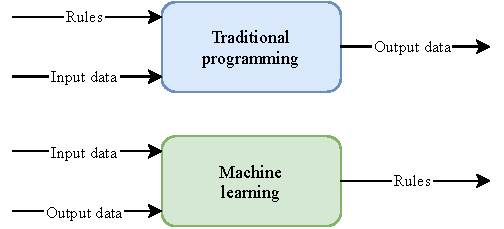
\includegraphics[width=0.7\textwidth]{thesis/figures/ml-versus-tradional-programming_cropped.pdf}
    \caption{Traditional programming compared to machine learning.}
    \label{fig:ml-versus-tradional-programming}
\end{figure}

In this thesis, we will in particular look at two approaches for ML, namely \textit{supervised} and \textit{unsupervised learning}. In a supervised learning setting, we give the ML program its input and output data. The goal is to learn the parameters of the ML program to map the input data to the output data. In an unsupervised learning setting, however, we do not give the ML program any output data, leaving the ML program to find structure in its input data. The goal of unsupervised ML programs is to discover and learn hidden patterns from the input data, by applying (possibly) several methods. In this thesis, we will learn from data by mainly using unsupervised ML methods (e.g. cluster analysis and dimensionality reduction in \cref{sec:analysis-of-word-embeddings-word-clustering}), but also some supervised ML methods (e.g. supervised polysemy prediction in \cref{sec:analysis-of-embeddings-supervised-polysemy-prediction}) as well. In the following subsections, we will introduce and explain general methods and concepts from machine learning.

\subsection{Clustering algorithms}
\label{sec:clustering-algorithms}
In a supervised machine learning setting, we typically use data $X$ and its associated labels $y$. The supervised task is to train a model to predict the labels $y$ using the data $X$. A classical example of a supervised machine learning task is to distinguish between dogs and cats, where $X$ is an image of a dog or a cat and the labels $y$ indicate whether or not the data $X$ represents a dog ($y=0$) or a cat ($y=1$). In an unsupervised setting, however, the labels $y$ are less likely to be present. To predict the labels $y$, we apply \textit{clustering algorithms}.

Clustering is one of the most important methods in unsupervised machine learning. Clustering algorithms divide some data $X$ into clusters (groups) such that the data in each cluster are similar in some sense. An example of this is clustering by using \textit{Euclidean distance}, which measures the distance of a line segment between two points $u$ and $v$. More formally, we define the Euclidean distance between two points $u$ and $v$ as
\begin{align}
    d(u, v) = ||u-v||_2 = \sqrt{\enclp{u_1 - v_1}^2 + \enclp{u_2 - v_2}^2 + \ldots + \enclp{u_n - v_n}^2},
    \label{eqn:euclidean-distance}
\end{align}
where $u$ and $v$ are two $n$-dimensional vectors. If we cluster by Euclidean distance, we want the distance between any two data points belonging to the same cluster to be small. We refer to this distance as the \textit{intracluster distance} or \textit{compactness}. Unfortunately, it is usually not enough to only minimize the intracluster distance; we also have to ensure that the distance between the clusters is as large as possible. To measure the distance between two clusters we measure the distance between two data points belonging to different clusters. We refer to this distance as the \textit{intercluster distance} or \textit{separation}. If a clustering algorithm can create clusters such that we have small intracluster distance and large intercluster distance, it indicates that the clustering algorithm is good for the data at hand. We note, however, that data can be complex and it can be hard to find good clusters. In the following sub-subsections, we look at some common clustering algorithms, explain how they work, and discuss their strengths/weaknesses. In each of the clustering algorithms, we assume that we have some data $X = \enclc{x_1, x_2, \ldots, x_n} \in \R^{n \times d}$. Furthermore, we will use the clustering algorithms below in the analysis of word embeddings (\cref{sec:word-embeddings}) in \cref{chap:analysis-of-word-embeddings}.

\subsubsection{k-means clustering}
\label{sec:k-means-clustering}
The \textit{k-means clustering} method is an unsupervised machine learning algorithm for identifying clusters in data \cite[Section 9.1]{bishop2006}. The algorithm uses an iterative approach to search for $k$ clusters, where $k$ is a \textit{hyperparameter} (i.e. in control by user). There exist several variants of this algorithm and we discuss two of them in later sub-subsections (see \cref{sec:mini-batch-k-means-clustering} and \cref{sec:k-medoids-clustering}). Following, we explain the standard (and naïve) variant of the algorithm (i.e. \textit{Lloyd's algorithm}), and we base this sub-subsection on \cite[Section 9.1]{bishop2006}.

The standard k-means clustering algorithm works as follows. The first step is to determine the initial cluster means, or \textit{centroids}. Since we want the algorithm to output $k$ clusters, we have to decide $k$ initial centroids. The simplest way to do this is to select $k$ random data points to be the initial $k$ centroids. The next step is to calculate the Euclidean distance between each data point to the cluster centroids. We do so because we want to determine which cluster each data point belongs to. Furthermore, we assign each data point to its closest cluster centroid and compute the mean of each cluster. The third and final step is to move the cluster centroid to the new mean of each cluster. We repeat the second and third steps until convergence is met (e.g. change of loss is less than a set threshold). Finally, we illustrate the use of k-means clustering in \cref{fig:k-means-clustering-2d-example}, where we see its cluster boundaries, representing the clusters. The white crosses represent the cluster centroids.
\begin{figure}[H]
    \centering
    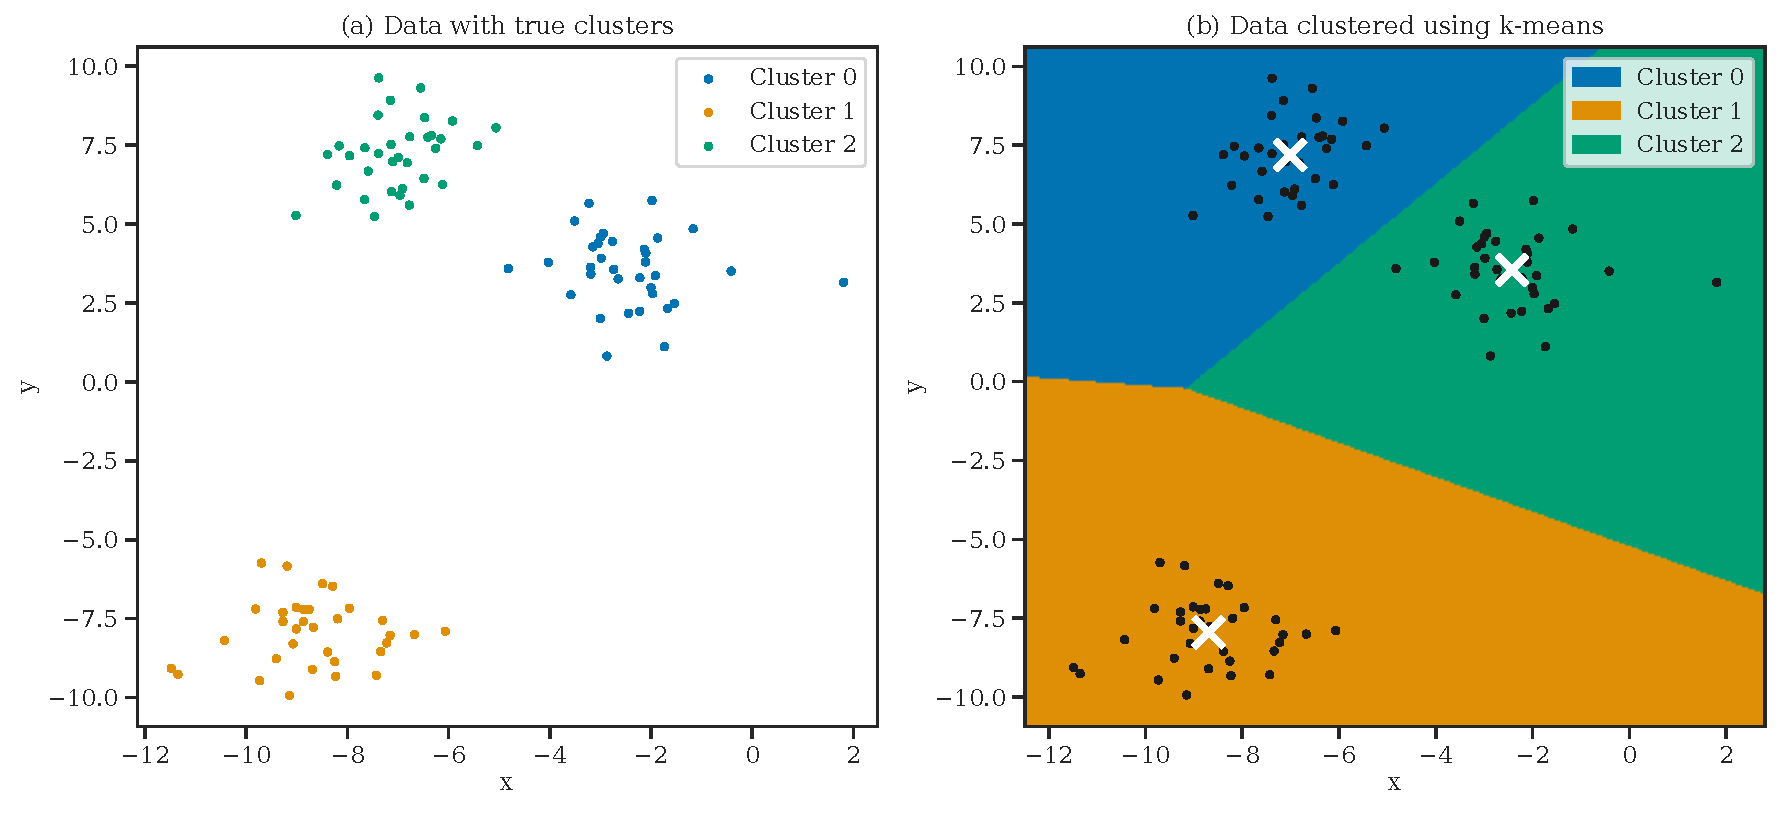
\includegraphics[width=\textwidth]{thesis/figures/k-means-clustering-2d-example.pdf}
    \caption{Example of clustering using k-means clustering on a 2-dimensional data set with 3 clusters. We show the cluster boundaries in (b), emphasized by the colours. The white crosses represent the cluster centroids.}
    \label{fig:k-means-clustering-2d-example}
\end{figure}

Mathematically, the goal of k-means clustering is to minimize the squared distance between the points in each cluster to its respective centroid, which we refer to as the within-cluster sum of squares (WCSS). The objective is to find
\begin{align}
    \argmin_{C} \sumlim{i=1}{k} \sumlim{x \in C_i}{} \norm{x - \mu_i}^2,
\end{align}
where $C = \enclc{C_1, C_2, \ldots, C_k}$ are the clusters of the data $X$, $k$ is a hyperparameter for the number of clusters and $\mu_i$ is the cluster centroid of cluster $C_i$.

The main advantage of k-means clustering is its simplicity, both in implementation and when interpreting the results. The algorithm also scales well to larger data sets, and there is only one hyperparameter to tune (number of clusters $k$). As for the disadvantages, the algorithm is rather sensitive to the initialization of centroids in the first step. If we were to select bad initial centroids, the convergence time of the algorithm increases greatly, and we might end up with bad clusters. We also have to choose the number of clusters manually, which is a downside if we have no additional knowledge of the data beforehand. In addition to this, the algorithm suffers from the \textit{curse of dimensionality}, which is a set of problems that can occur when analyzing high-dimensional data (i.e. greater than two to three dimensions). In the context of k-means clustering, as the dimensionality increases, it becomes more and more difficult to distinguish between data points (all points converge to the same distance). We illustrate an effect of the curse of dimensionality in \cref{fig:curse-of-dimensionality}.
\begin{figure}[H]
    \centering
    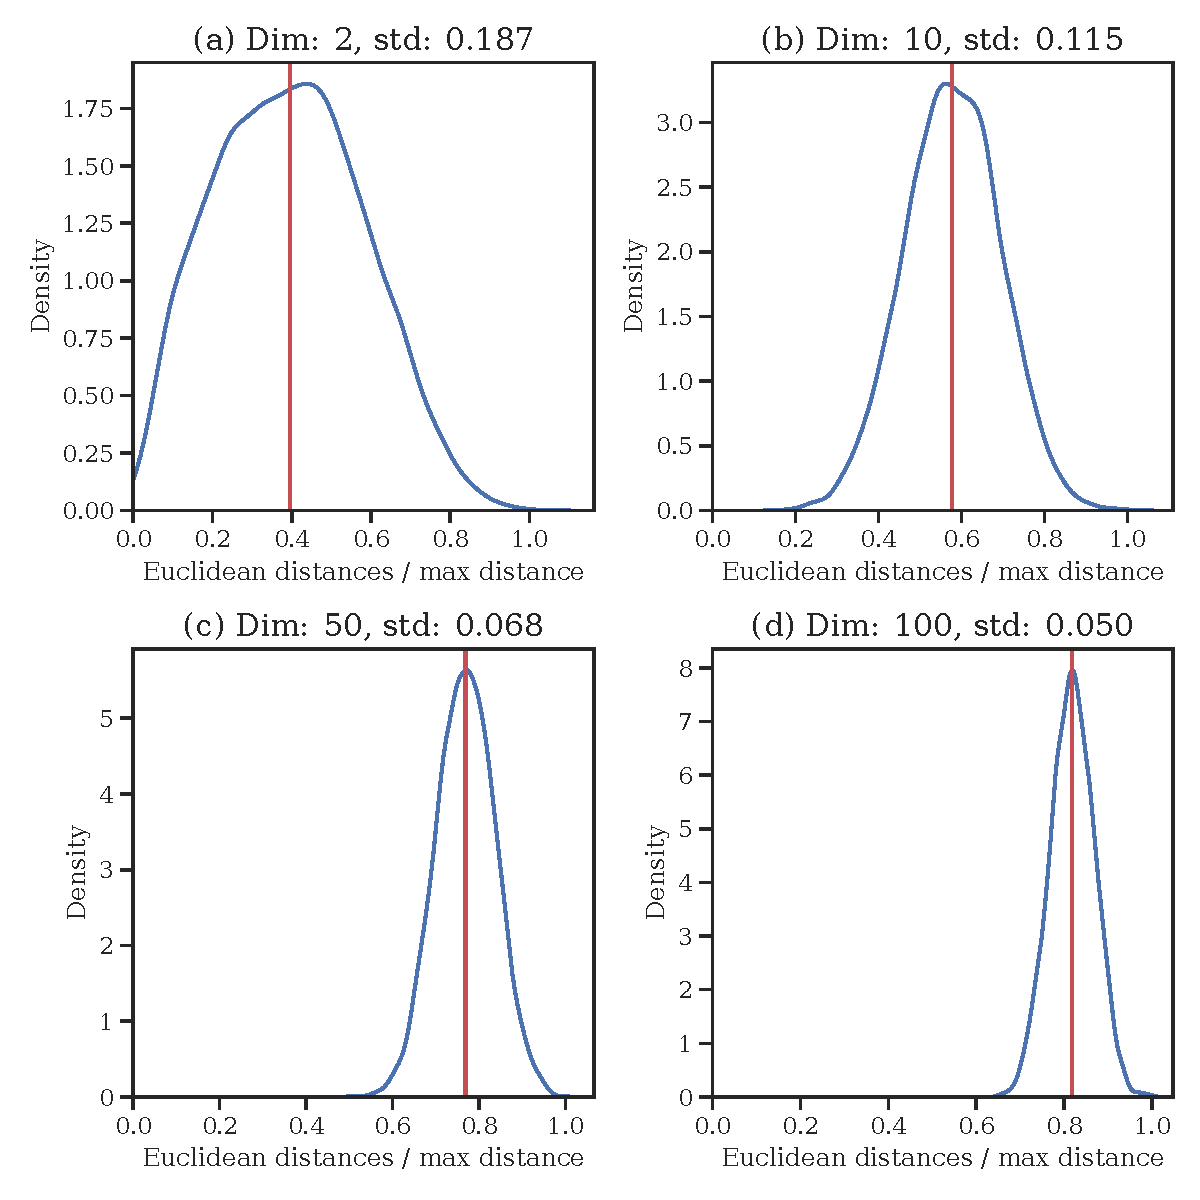
\includegraphics[width=0.9\textwidth]{thesis/figures/curse-of-dimensionality.pdf}
    \caption{Four illustration plots showing an effect of the curse of dimensionality. The distance between points in higher dimensional spaces becomes the same as the dimensionality increases, and thus, it is harder to differentiate between points using distance metrics. The blue line represents the density of the pairwise Euclidean distances (we divide by the max distance to normalize the x-axis). The red line is the mean distance.}
    \label{fig:curse-of-dimensionality}
\end{figure}

\subsubsection{Mini-batch k-means clustering}
\label{sec:mini-batch-k-means-clustering}
\textit{Mini-batch k-means clustering} is a variant of k-means clustering, where we use \textit{mini-batches} of data points to find a suitable clustering \cite{sculley2010}. To create the mini-batches, we randomly sample subsets of the training data for each training iteration (similar to the mini-batches in gradient descent from \cref{sec:ann-optimizers}). We refer to \cite{sculley2010} when explaining mini-batch k-means clustering.

The algorithm is similar to the standard k-means clustering algorithm and comprises two major steps. In the first step, we initialize $k$ cluster centroids and sample $B=\enclc{b_1, b_2, \ldots, b_m} \subset X$ points at random from the data set $X$, where $m$ is the mini-batch size. In the second step, we update the cluster centroids by gradually moving the centroids. For each sample $b$ in the mini-batch, we update the centroids by taking the average of $b$ and the previous points assigned to the centroid. By doing so, we move the centroid with a decreasing rate over time. We repeat the first and second steps until convergence is met (e.g. change of loss is less than a set threshold).

The main advantage of mini-batch k-means clustering over standard k-means is that the convergence time is lower. By using mini-batches, we drastically reduce the computational requirement for converging to a local solution and, the results of mini-batch k-means clustering tend to only be slightly worse than the standard algorithm.

\subsubsection{k-medoids clustering}
\label{sec:k-medoids-clustering}
\textit{K-medoids clustering} is an alternative to the standard k-means clustering algorithm \cites{Kaufman1990}[p. 427 - 428]{bishop2006}. K-medoids clustering uses data points for its cluster centroids and works with any dissimilarity measure. A \textit{medoid} of a cluster is a data point where the average dissimilarity between the medoid and all other data points in the same cluster is minimal. We refer to \cites{Kaufman1990}[p. 427 - 428]{bishop2006}\, when explaining k-medoids clustering.

To solve the k-medoids problem efficiently, we use the \textit{Partitioning Around Medoids} (PAM) algorithm. Similar to the standard k-means clustering algorithm, PAM consists of two main stages, namely the \textit{build-} and \textit{swap} stages. In the build stage, we greedily select $k$ of the $n$ data points to be the initial cluster medoids, which we denote $M = \enclc{m_1, m_2, \ldots, m_k} \subset X$. To select $M$ initially, we want to minimize the dissimilarity between the cluster medoids and points in the same cluster. In other words, initially, we set the first medoid $m_1$ to be the data point such that the dissimilarity between then medoid and all other data points is minimal. Then, for all proceeding medoids ($m_2, \ldots, m_k$), we look for medoids such that the dissimilarity between the additional medoid, the data points in the same cluster as the new medoid, and all other medoids (and its cluster data points) is minimal. We repeat this process until we have $k$ medoids. Following, the swap stage consists of iteratively swapping out the $k$ medoids with other data points from the data set, if it minimizes the overall dissimilarity. The algorithm terminates if by swapping the medoids with other data points we do not get lower dissimilarity. Finally, we illustrate the use of k-medoids clustering in \cref{fig:k-medoids-clustering-2d-example}, where we see that each point is connected to its cluster by a line, signalizing the dissimilarity between the points and the cluster medoids. The black dots represent the cluster medoids.
\begin{figure}[H]
    \centering
    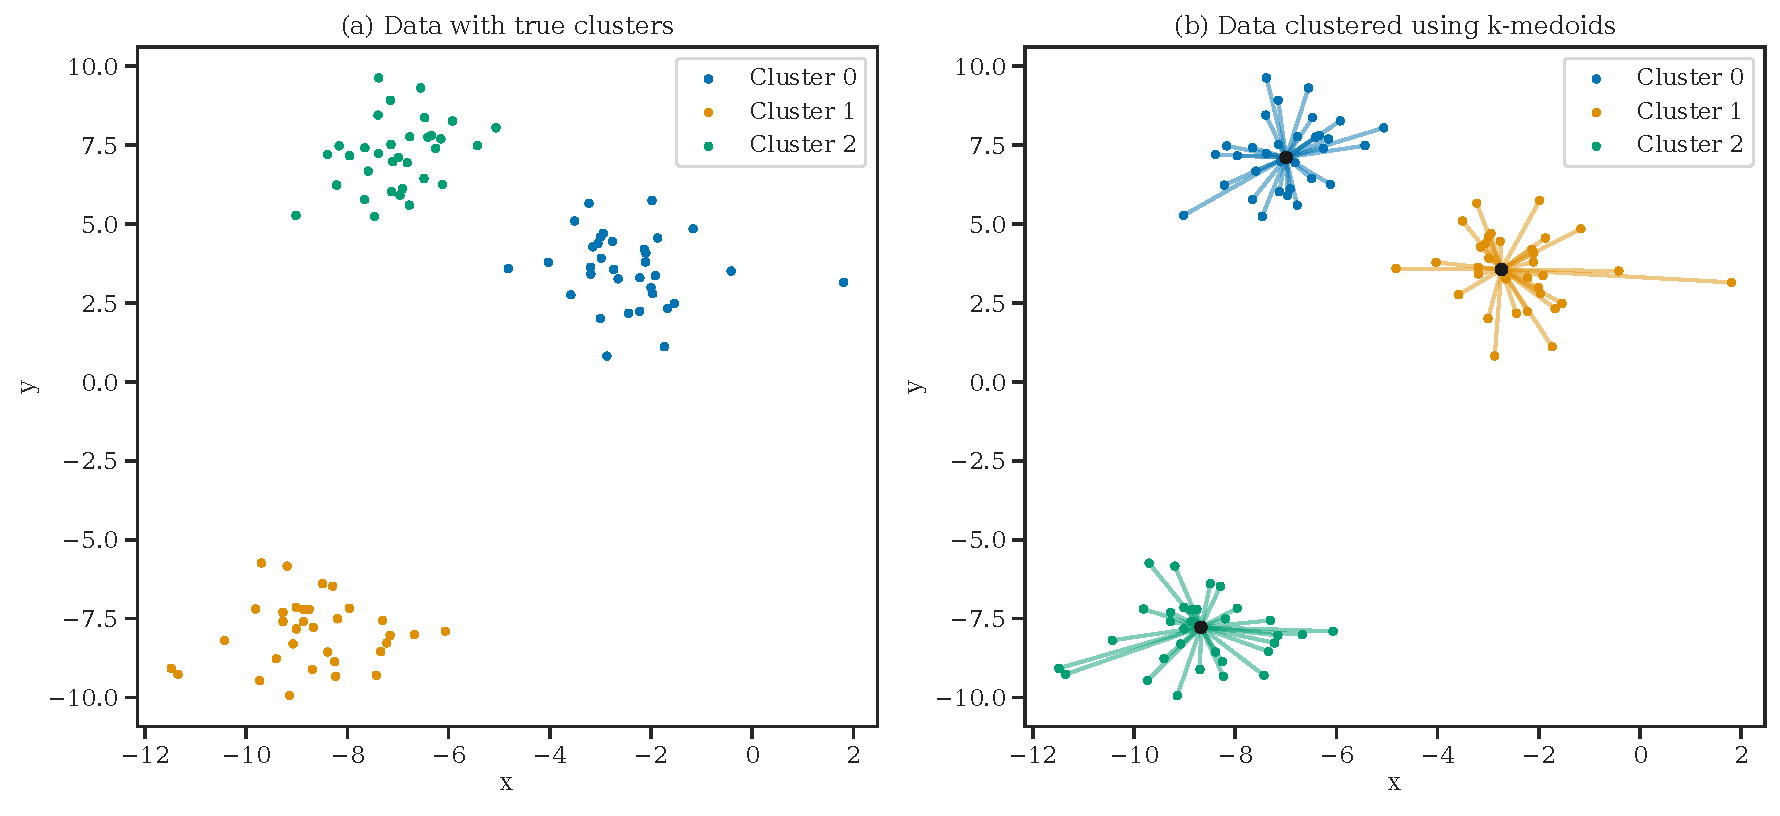
\includegraphics[width=\textwidth]{thesis/figures/k-medoids-clustering-2d-example.pdf}
    \caption{Example of clustering using k-medoids clustering on a 2-dimensional data set with 3 clusters. The lines signalize dissimilarity between points and the cluster medoids.}
    \label{fig:k-medoids-clustering-2d-example}
\end{figure}

The main advantage of k-medoids is that it is more interpretable and robust to outliers than the standard k-means clustering algorithm since it uses actual data points as centroids. In addition to this, we may use any dissimilarity measure, whereas, in the standard k-means clustering, Euclidean distance is the only option. Even though k-medoids clustering seems to be the superior choice over k-means clustering, it suffers from the fact it is more computationally heavy to compute and thus is not always feasible to run for large data sets.

\subsubsection{Gaussian mixture models}
\label{sec:gmm-clustering}
\textit{Gaussian mixture models} (GMMs) are probability distributions which consists of a mixture of multiple \textit{Gaussians} \cite[Section 9.2]{bishop2006}. A Gaussian (i.e. normal) is a probability distribution which was several nice properties, such as mean as its mode and symmetry. In the context of cluster algorithms, we use GMMs to cluster data points by using multivariate (i.e. of higher dimension) Gaussian distributions as cluster centroids. In particular, for each cluster centroid $c_i, 1 \leq i \leq k$, we define $\mu_i$ to be the cluster mean, $\Sigma_i$ to be the cluster covariances and $\pi_i$ to be the \textit{mixing coefficients}. The cluster means $\mu_i$ and covariances $\Sigma_i$ determines the localization and spread for each cluster, while the mixing coefficients $\pi_i$ determine how much we emphasize each cluster. To estimate the parameters $\theta = \enclc{\mu, \Sigma, \pi}$ of GMMs, we use the Expectation-Maximization (EM) algorithm, which is an iterative algorithm. When explaining GMMs and the EM algorithm, we refer to \cite[Section 9.2]{bishop2006}.

The EM algorithm starts by initializing its parameters $\mu$, $\Sigma$, and $\pi$. There exist several methods for initializing the parameters and it is common to first run k-means clustering on the data to obtain a suitable starting point. By running k-means clustering first, we compute the initial parameters by using statistics from the result of k-means. Furthermore, the EM algorithm consists of two main stages, namely \textit{expectation} and \textit{maximization}. In the expectation stage, we compute the responsibilities for each data point in $X$ using the current set of parameters. With responsibilities, we mean how much each Gaussian is responsible for explaining a single data point in $X$. Next, in the maximization step, we use the responsibilities from the expectation step to update the parameters such that the likelihood $\text{P}(X | \theta)$ is maximal. The likelihood $\text{P}(X | \theta)$ tells us how good the set of parameters $\theta$ fits our data $X$. The exact derivation and update rules for each parameter are left out and we refer the reader to \cite[Section 9.4]{bishop2006} for more details. Once a suitable threshold is met with respect to $\text{P}(X | \theta)$, the algorithm terminates and we converge to a set of parameters $\hat{\theta}$. Using the final parameters, $\hat{\theta}$, we predict which Gaussian (i.e. cluster) to associate for every data point $x \in X$, by selecting the Gaussian with the highest density. Finally, we illustrate the effect of GMM clustering in \cref{fig:k-gmm-clustering-2d-example}, where we see that the different clusters have different shapes (i.e. means and covariances).
\begin{figure}[H]
    \centering
    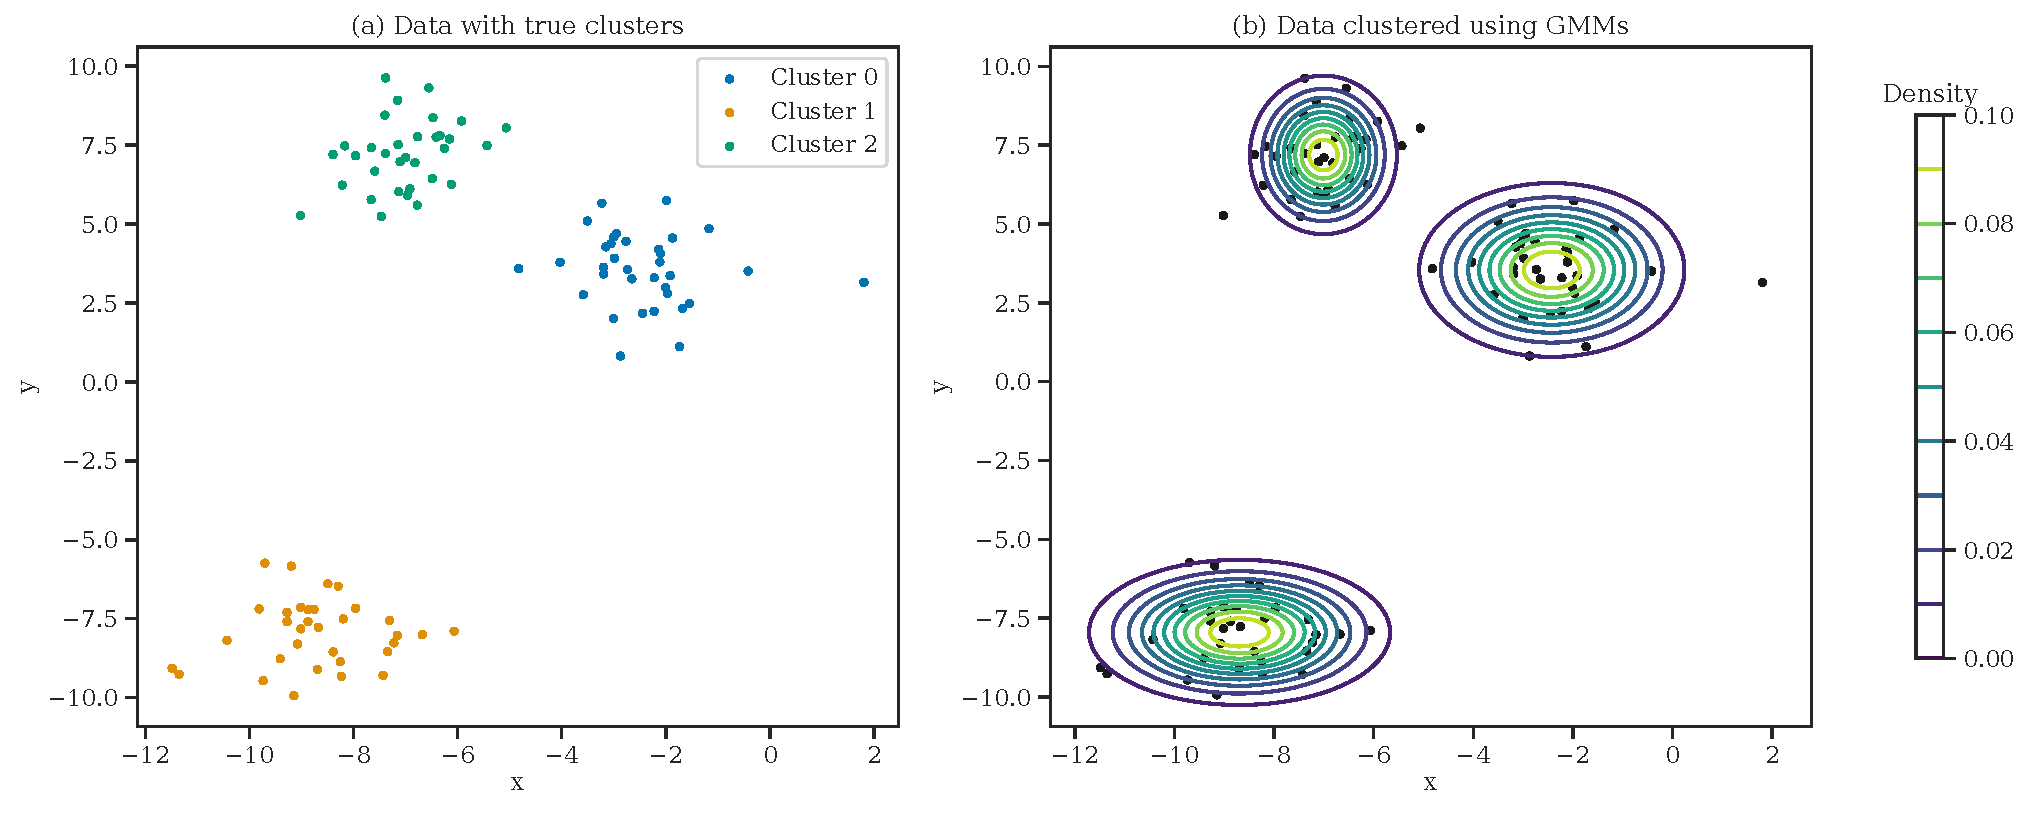
\includegraphics[width=\textwidth]{thesis/figures/k-gmm-clustering-2d-example.pdf}
    \caption{Example of clustering using GMMs on a 2-dimensional data set with 3 clusters. The different clusters have different shapes, as shown by the ellipsoids.}
    \label{fig:k-gmm-clustering-2d-example}
\end{figure}

The main advantage of using GMMs is that clusters can be of different shapes and we get a probabilistic measure of which cluster each data point belongs to (i.e. fuzzy clustering). The convergence time of GMMs depends on the initialization of the parameters $\theta$. If we use k-means clustering to initialize the parameters $\hat{\theta}$, then the overall convergence time is greater than simply running k-means alone. On the other hand, if we use a completely random initialization of the parameters $\theta$, then the GMMs converges a lot faster at the risk of converging in a bad local maximum, leading to worse results.

\subsubsection{Hierarchical clustering}
\label{sec:hierarchical-clustering}
\textit{Hierarchical clustering} is a group of clustering algorithms that constructs clusters by recursively partitioning the data points of $X$ in top-down or bottom-up fashion \cite{Rokach2005}. We divide the two methods of hierarchical clustering into what we call \textit{agglomerative} and \textit{divisive hierarchical clustering}. Furthermore, we base this sub-subsection on \cite{Rokach2005}.

Using the agglomerative hierarchical clustering, each data point in $X$ starts in its own cluster and we successively merge them until all points are in their own respective clusters. In contrast to the agglomerative method, divisive hierarchical clustering starts with all data points in $X$ in a single cluster. Then, we divide the single cluster into smaller clusters, until each point is in its own cluster. Following, we call the output of a hierarchical clustering algorithm a \textit{dendrogram}. We use dendrograms to represent the clustering tree structure. We illustrate an example of a dendrogram in \cref{fig:dendrogram-example}.
\begin{figure}[H]
    \centering
    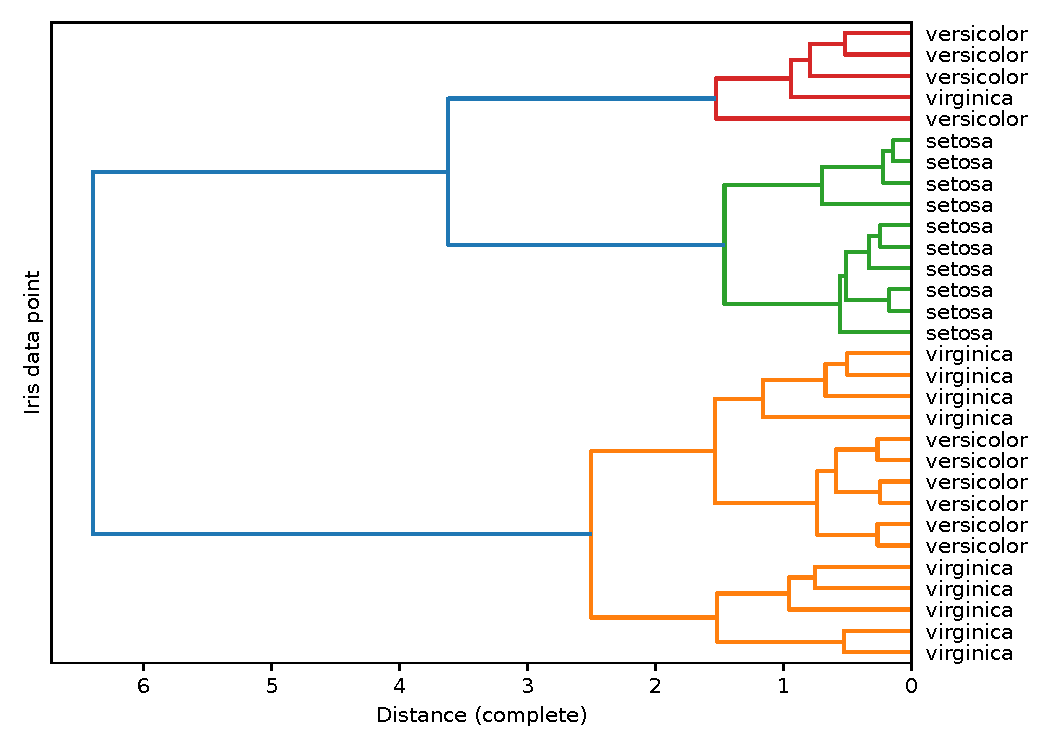
\includegraphics[width=0.9\textwidth]{thesis/figures/dendrogram-example.pdf}
    \caption{Complete-linkage clustering on a subset of the Iris data set \cite{Anderson1936,Fisher1936}, showing its dendrogram.}
    \label{fig:dendrogram-example}
\end{figure}

To merge or divide clusters, we use some similarity measure to either merge similar data points (agglomerative) or divide dissimilar data points (divisive). Exactly which data points we choose to merge or divide depends on which criterion we want to optimize. There exist several different criteria we may choose to perform hierarchical clustering. Below we list some of the most common ones and mention some pros/cons for each criterion.
\begin{itemize}
    \item \textbf{\textit{Single-linkage} clustering} --- combines two clusters that contain the closest pair (i.e. largest similarity) of elements that do not yet belong to the same cluster as each other.
    \begin{itemize}
        \item Single-linkage clustering tends to produce clusters of long chains, which can lead to the clustering of data points which in reality are far apart from each other.
        \item Single-linkage clustering is fast to use for big data sets and can create clusters of different shapes and sizes.
        \item Single-linkage clustering is sensitive to noise.
    \end{itemize}
    \item \textbf{\textit{Complete-linkage} clustering}  --- combines two clusters that contain the furthest pair (i.e. smallest similarity) of elements that do not yet belong to the same cluster as each other.
    \begin{itemize}
        \item Complete-linkage clustering has bias towards spherical clusters.
        \item Complete-linkage clustering works well on data with noise.
        \item Complete-linkage clustering tends to split large clusters.
    \end{itemize}
    \item \textbf{\textit{Average-linkage} clustering} --- combines two clusters such that the average pairwise distance of the new cluster is minimum.
    \begin{itemize}
        \item Average-linkage clustering has bias towards spherical clusters.
        \item Average-linkage clustering works well on data with noise.
    \end{itemize}
    \item \textbf{\textit{Ward-linkage} clustering} --- combines two clusters such that the variance of the new cluster is minimum \cite{Ward1963}.
    \begin{itemize}
        \item Ward-linkage clustering has bias towards spherical clusters.
        \item Ward-linkage clustering works well on data with noise.
    \end{itemize}
\end{itemize}

Overall, hierarchical clustering is a great clustering algorithm for partitioning the data in a tree fashion. By performing hierarchical clustering, we use the resulting dendrogram to determine the number of clusters by cutting it at a certain distance threshold. In the example from \cref{fig:dendrogram-example}, a suitable cut could be at distance equal to 3, leading to 3 clusters. In addition to this, different choices of linkages can lead to different clusterings. For this reason, we should test multiple linkages to figure out what fits the data the most.

\subsubsection{Spectral clustering}
\label{sec:spectral-clustering}
\textit{Spectral clustering} is a clustering algorithm that first reduces the dimensionality of the data set and then applies a clustering algorithm \cite{Andrew2002}. In particular, spectral clustering uses the eigenvalues of the \textit{affinity matrix} (e.g. a similarity matrix using pairwise Euclidean distances) of the data $X$ to reduce its dimensionality before applying some common clustering algorithm, such as k-means clustering (see \cref{sec:k-means-clustering}). We base this sub-subsection on \cite{Andrew2002}.

Imagine that we want to cluster the data into $k$ clusters. Spectral clustering starts with the construction of the affinity matrix $A$. We typically use some similarity measure to create pairwise distances between data points to create such an affinity matrix. Then, we compute the \textit{graph Laplacian} $L = D - A$, where $D$ is a diagonal matrix with $D_{ii} = \sumlim{j}{} A_{ij}$ and $A$ is the affinity matrix. The graph Laplacian $L$ is simply a matrix representation of a graph, and in our case, the similarities between data points in $X$. Next, we compute the eigenvectors of $L$, and using these eigenvectors we get a lower-dimensional space of the original data $X$ (from $d$ dimensions to $k$). Finally, we use a clustering algorithm, such as k-means clustering, on the eigenvectors of $L$ to get the final clustering.

The main advantage of spectral clustering is that it performs a dimensionality reduction on the data before applying a clustering algorithm. The dimensionality reduction can make the clustering algorithm less prone to noise and yield better results. Unfortunately, the computational requirement of spectral clustering is rather high, and for big data sets, it is simply infeasible.

\subsubsection{HDBSCAN}
\label{sec:hdbscan-clustering}
Clusters come in different shapes and sizes, and real-life data is rather noisy. \textit{DBSCAN} is a density-based algorithm that handles clusters of different shapes and sizes and is robust to noise \cite{Ester1996}. It, however, is only able to produce a "flat" clustering using some global threshold parameter. \textit{HDBSCAN} is a generalization of DBSCAN and improves on it by creating a complete density-based clustering hierarchy \cite{Campello2013}, automatically extracting flat clusters. HDBSCAN is different from the other clustering algorithms we have seen so far, as it can perform clustering without predetermining the number of clusters beforehand and can mark data points a noise. To fully understand the HDBSCAN algorithm, we introduce its key concepts and then explain how the algorithm works in practice. We base this sub-subsection on the "How HDBSCAN Works" article from \cite{how-hdbscan-works-2016}.

HDBSCAN is a density-based clustering algorithm and, for this reason, requires an inexpensive density estimation method to be efficient. Using k-nearest neighbours, the authors of HDBSCAN estimate the density efficiently. In particular, we first define the \textit{core distance} of a data point $x \in X$ to be the distance to the $\textit{minPts}$-nearest neighbour (including $x$), which we denote $d_{core}(x)$. $\textit{minPts}$ is a hyperparameter and controls how conservative we want the clustering to be; the larger $\textit{minPts}$, the more "noisy" data points. To further spread apart data points that have low density, we define the \textit{mutual reachability distance} metric (MRD) as
\begin{align}
    d_{mreach}(x, y) = \max \enclc{ d_{core}(x), d_{core}(y), d(x, y) },
    \label{eqn:mutual_reachability_distance}
\end{align}
where $d(x, y)$ is the distance between data point $x$ and data point $y$ using the original distance metric. Under the MRD metric, data points in dense regions do not change their distances, but for sparse data points, the distances change such that they are at least their core distance to other points.

Next, using the MRD metric, we find dense areas in the data. To find such areas, we create a \textit{minimal spanning tree} (MST) where each node represents a data point $x \in X$ and edges connecting pairs of nodes has a weight equal to the MRD between the two nodes. By using an MST, we get a graph with the minimal set of edges between nodes such that the weight between the nodes is minimal. Additionally, if we drop exactly one edge of the graph, we disconnect it; for each pair of nodes, we connect them by exactly one edge. Using these two facts, we create a clustering hierarchy in a single-linkage clustering manner. First, we sort the weights of the edges of the MST in increasing order. Following, we iterate over the edges of the MST and merge data points into clusters (note that each data point is its own cluster initially). Now, from the hierarchical clustering, we are left with a dendrogram, which we illustrate in \cref{fig:hdbscan-dendrogram-example}. We are now are left with a critical question: How should we define the cut to get a flat clustering?
\begin{figure}[H]
    \centering
    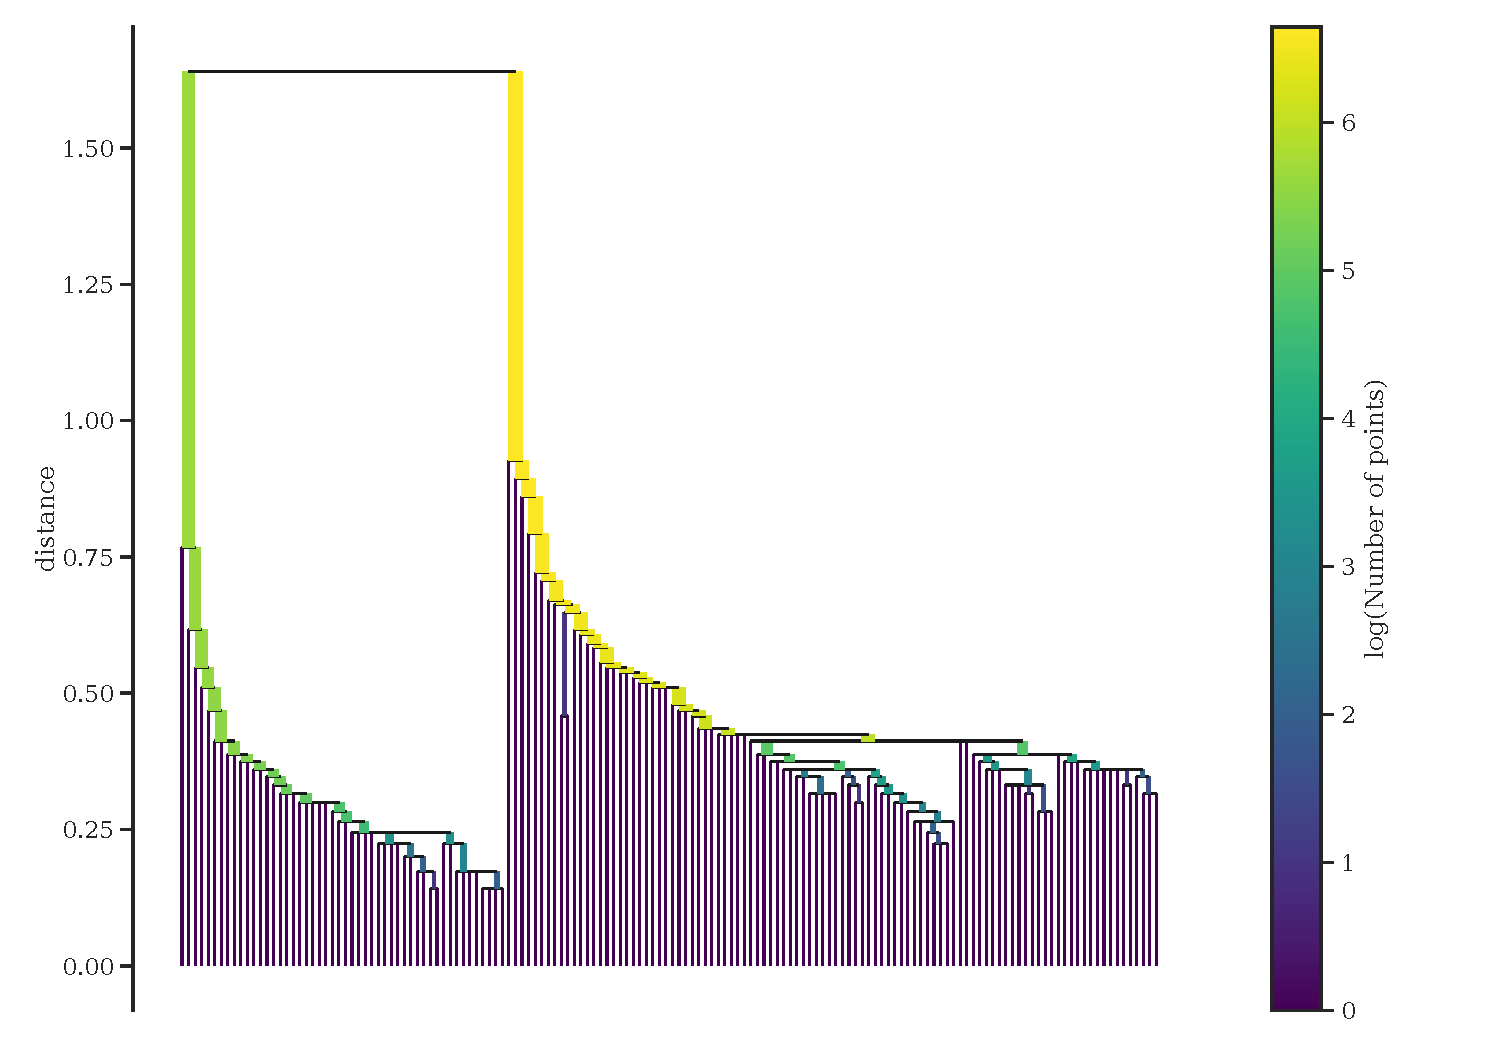
\includegraphics[width=0.8\textwidth]{thesis/figures/hdbscan-single-linage-tree-example.pdf}
    \caption{Single-linkage dendrogram plot from HDBSCAN on the Iris data set \cite{Anderson1936,Fisher1936}.}
    \label{fig:hdbscan-dendrogram-example}
\end{figure}

Dendrograms can be difficult to interpret, especially once we reach a certain number of data points. For this reason, the authors of HDBSCAN \textit{condense} (or \textit{compact}) the dendrogram from the hierarchical clustering such that they obtain a flat clustering. First, we define the notion of \textit{minClusterSize}, which is a hyperparameter controlling the minimal cluster size at any time. Following, we walk down the dendrogram, starting from the root cluster, and at each split, we check whether or not the new cluster has at least \textit{minClusterSize} data points in it. If the new cluster has at least \textit{minClusterSize} data points in it, we let that cluster be in the tree. If the new cluster has less than the \textit{minClusterSize} in it, then we let the parent cluster identify the new cluster and we remove the node from the tree. As we walk through the dendrogram to condense it, we also include at what distance clusters merge into the parent cluster, i.e. "fall out of clusters". We illustrate with an example of a condensed dendrogram in \cref{fig:hdbscan-condensed-dendrogram-example}.
\begin{figure}[H]
    \centering
    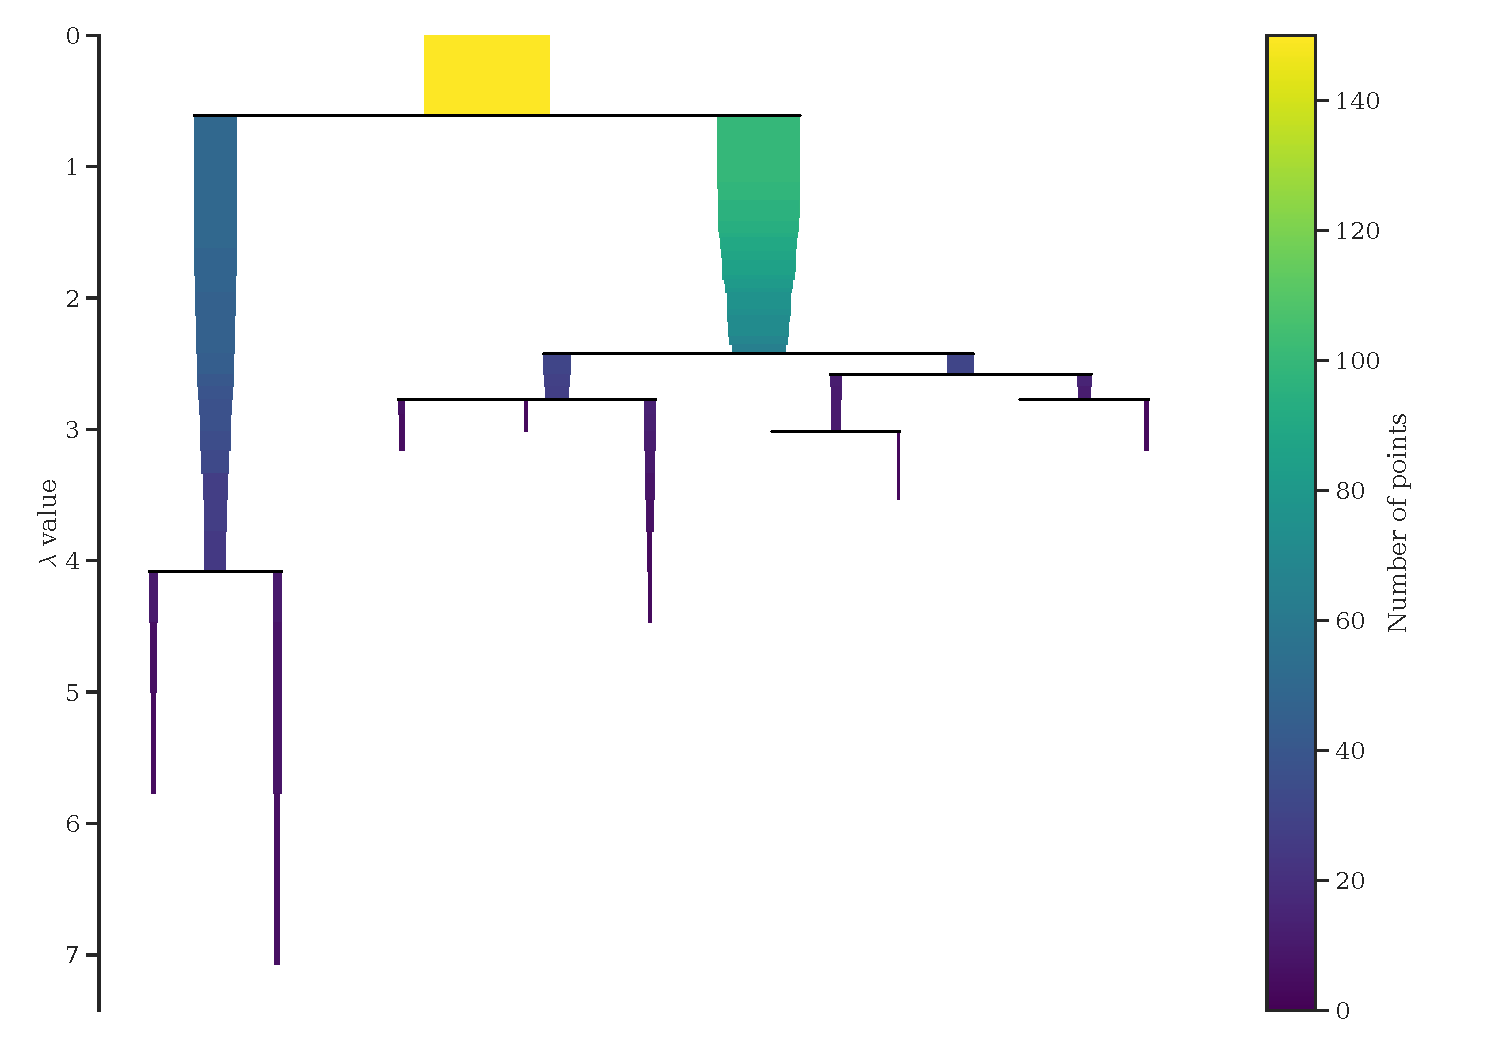
\includegraphics[width=0.8\textwidth]{thesis/figures/hdbscan-condensed-tree-example.pdf}
    \caption{Condensed dendrogram plot from HDBSCAN on the Iris data set \cite{Anderson1936,Fisher1936}.}
    \label{fig:hdbscan-condensed-dendrogram-example}
\end{figure}

Now, to define the flat cut in a condensed diagram, we select the clusters such that the largest total area of "ink" is maximal, under an additional constraint that we do not select clusters that are descendants of an already selected cluster. Furthermore, we mark any clusters which we do not select in the previous step as noise, as they are merely artefacts of the initial hierarchical clustering. We then decide the final clustering, which we illustrate in \cref{fig:hdbscan-condensed-dendrogram-final-cut-example}.
\begin{figure}[H]
    \centering
    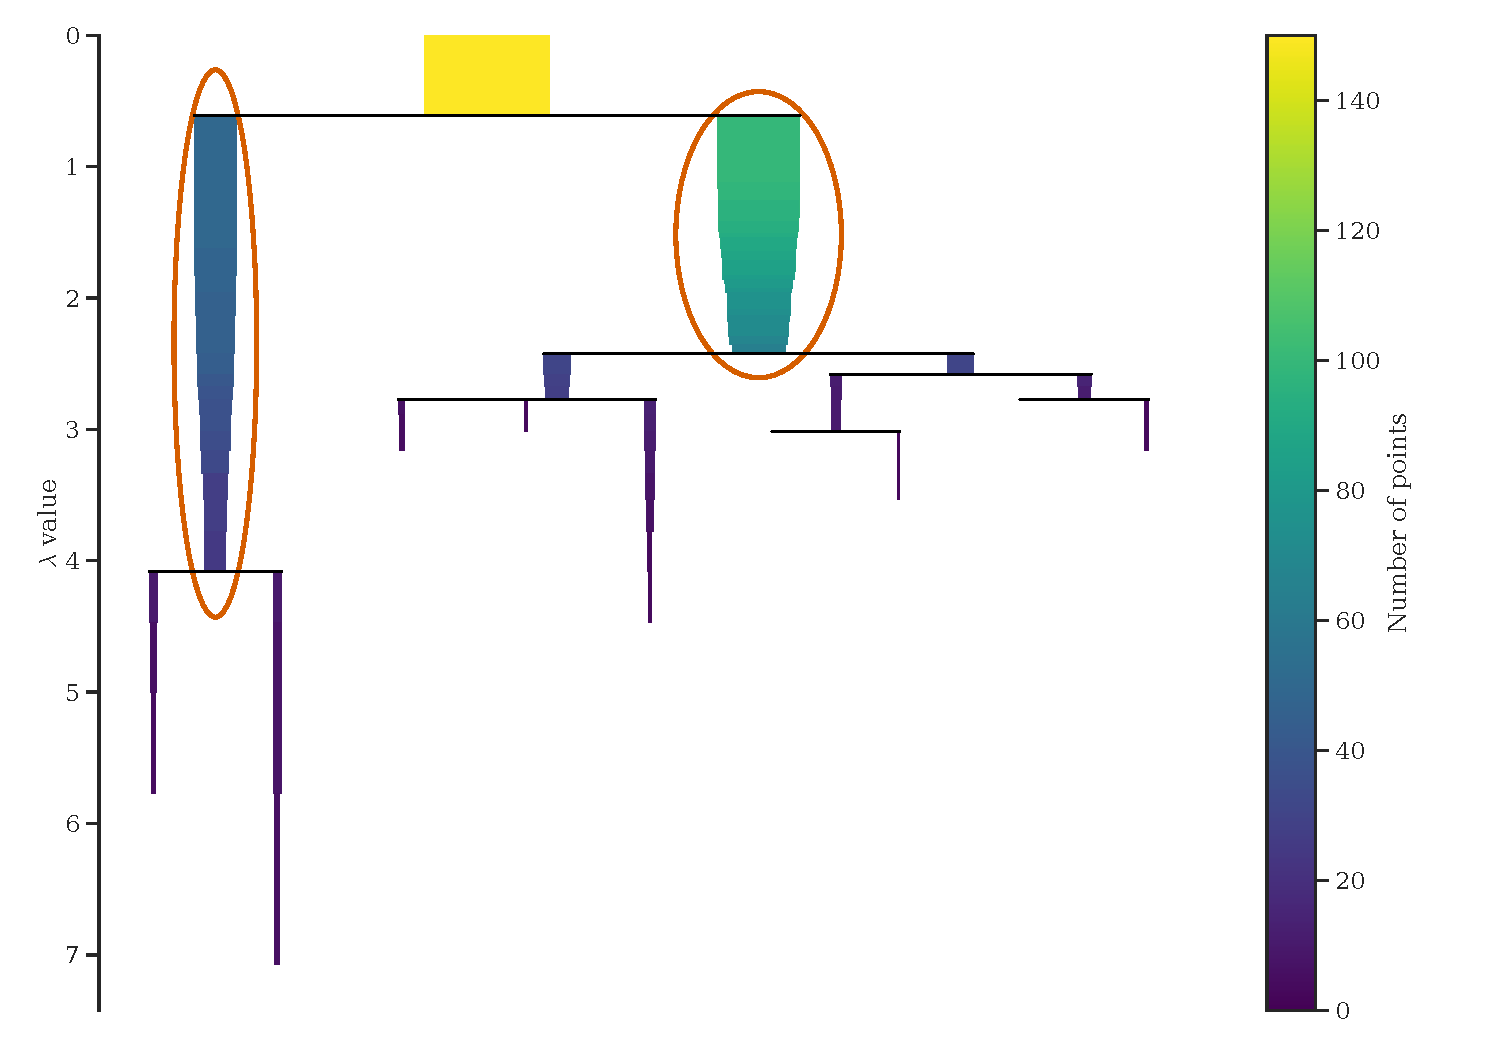
\includegraphics[width=0.8\textwidth]{thesis/figures/hdbscan-condensed-tree-final-cut-example.pdf}
    \caption{Condensed dendrogram plot from HDBSCAN on the Iris data set \cite{Anderson1936,Fisher1936}. We show the "final cut" in the red circles and consider all data points below the clusters with the red circles as noise.}
    \label{fig:hdbscan-condensed-dendrogram-final-cut-example}
\end{figure}

The main advantage of HDBSCAN is that it is able to find the number of clusters automatically, that we can have different shapes of clusters and are able to mark data points as noise. Dealing with noisy data points can be a challenge, and depending on how we treat them (exclusion, each noisy data point in its own cluster, etc.), it may lead to different results.

\subsubsection{ToMATo}
\label{sec:tomato-clustering}
\textit{Topological Mode Analysis Tool} (ToMATo) is a clustering algorithm that uses concepts from topological data analysis (TDA) \cite[p. 118-131]{Oudot2015}. In particular, ToMATo uses the concepts of persistence diagrams (see \cref{sec:persistence diagram}) and prominence to perform clustering. We divide the ToMATo clustering algorithm into three parts: density estimation and neighbour graph creation (1), mode-seeking (2) and merging (3). Furthermore, we refer to \cite[p. 118-131]{Oudot2015} when explaining the algorithm.

First (1), we use any density estimation scheme to estimate the density of our data. A common choice is to use kernel density estimation with some kernel (e.g. Gaussian). We denote the density of a data point $x_i \in X, i = 1, 2, \ldots, n$ as $\Tilde{f}(x_i)$. In addition to density estimation, we compute a neighbourhood graph $G$ to determine the neighbours of data points. In the graph $G$, each vertex is a data point and edges represent neighbours. To compute $G$, it is common to use a $k$-nearest neighbour graph, where $k$ represents the number of neighbours.

Using the density estimator $\Tilde{f}$ and neighbourhood graph $G$, we compute the initial clusters of ToMATo by performing mode-seeking (2). First, we sort the vertices of $G$ by decreasing $\Tilde{f}$-values and iterate over them. At each vertex $i$, compare the $\Tilde{f}$ values of vertex $i$ and its neighbours. If $\Tilde{f}(x_i)$ is greater than $\Tilde{f}$ of its neighbours, we then denote vertex $i$ as a peak of $\Tilde{f}$. Otherwise, we connect vertex $i$ to the neighbour with the greatest $\Tilde{f}$-value. By doing so, we create a spanning forest, where each spanning tree represents peaks of the underlying true density function. In the next step, we use this spanning forest and merge the trees to obtain a clustering.

The last step is the merging (3) of the spanning forest from (2). To do this, ToMATo iterates over the vertices of $G$ again (in the same order as in (2)) and we use a \textit{union-find} data structure to keep track of the spanning trees we merge. We denote the union-find data structure as $\mathcal{U}$. The entries $e \in \mathcal{U}$ correspond to the union of spanning trees. The root of an entry $r(e)$, is the vertex in $e$ whose $\Tilde{f}$-value is the highest, i.e. a local peak of $\Tilde{f}$ in $G$. Now, iterating over the vertices of $G$, we check whether or not vertex $i$ is a peak of $\Tilde{f}$. If vertex $i$ is a peak of $\Tilde{f}$, i.e. root of some spanning tree $S$, we create a new entry $e$ in $\mathcal{U}$, in which we store $S$. The root of entry $e$ is set to the vertex itself, i.e. $r(e) = i$. If vertex $i$ is not a peak of $\Tilde{f}$, it means that it belongs to some existing entry $e_i \in \mathcal{U}$ and we look for potential merges of $e_i$ with other entries in $\mathcal{U}$. In particular, we iterate over neighbours $e \in \mathcal{E}$, $e \neq e_i$, of $i$ in $G$ and check whether $\min \enclc{ \Tilde{f}(x_{r(e)}), \Tilde{f}(x_{r(e_i)}) } < \Tilde{f}(x_i) + \tau$, where $\tau$ is the \textit{prominence} threshold parameter. In other words, we check whether or not two entries have different $\Tilde{f}$-value and at least one of them has root with less than $\tau$ prominence. If this is true, we merge $e$ and $e_i$ into a single entry in $\mathcal{U}$, i.e. $e \cup e_i$, and we merge the entry with the lower root into the one with the higher root.

Once the merging step is complete, we are left with a union-find structure $\mathcal{U}$. For every entry $e$ of $\mathcal{U}$, we connect them to its parent entry $p(e)$ such that $\Tilde{f}(x_{p(e)}) > \Tilde{f}(x_e)$. In other words, by iteratively searching for the topmost parent, we determine which cluster we connect each entry (i.e. data point) to. We see the ToMATo clustering algorithm as a combination of mode-seeking (from step (2)) and hierarchical clustering (from step (3)). As a result of the hierarchical structure, we can visualize when entries in $\mathcal{U}$ merge into other entries, and thus, explain the lifespans of entries. More precisely, an entry in $\mathcal{U}$ is "born" when we create it in $\mathcal{U}$ and "dies" when we merge it into another entry with a higher root. Using persistence diagrams (see \cref{sec:persistence diagram}) we can explain the lifespans of entries and determine which entries live the longest (i.e. entries that never dies). We use the persistence diagram to determine which value for $\tau$ we should use. Different values of $\tau$ results in different numbers of clusters. In practice, let $\tau = +\inf$ and use the persistence diagram of $\mathcal{U}$ to find a suitable threshold $\hat{\tau}$ such that we get the number of clusters we want. Then, we run ToMATo again using $\hat{\tau}$ as the threshold parameter to get the final clustering. Finally, we motivate the use of ToMATo in \cref{fig:k-tomato-clustering-2d-example}, where we see from the persistence diagram in (b) that ToMATo found 5 clusters, but 3 of them are significantly far from the diagonal (i.e. high prominence). This indicates that the data set should consist of 3 clusters, and thus, we run ToMATo again setting the prominence threshold such that we get 3 clusters.
\begin{figure}[H]
    \centering
    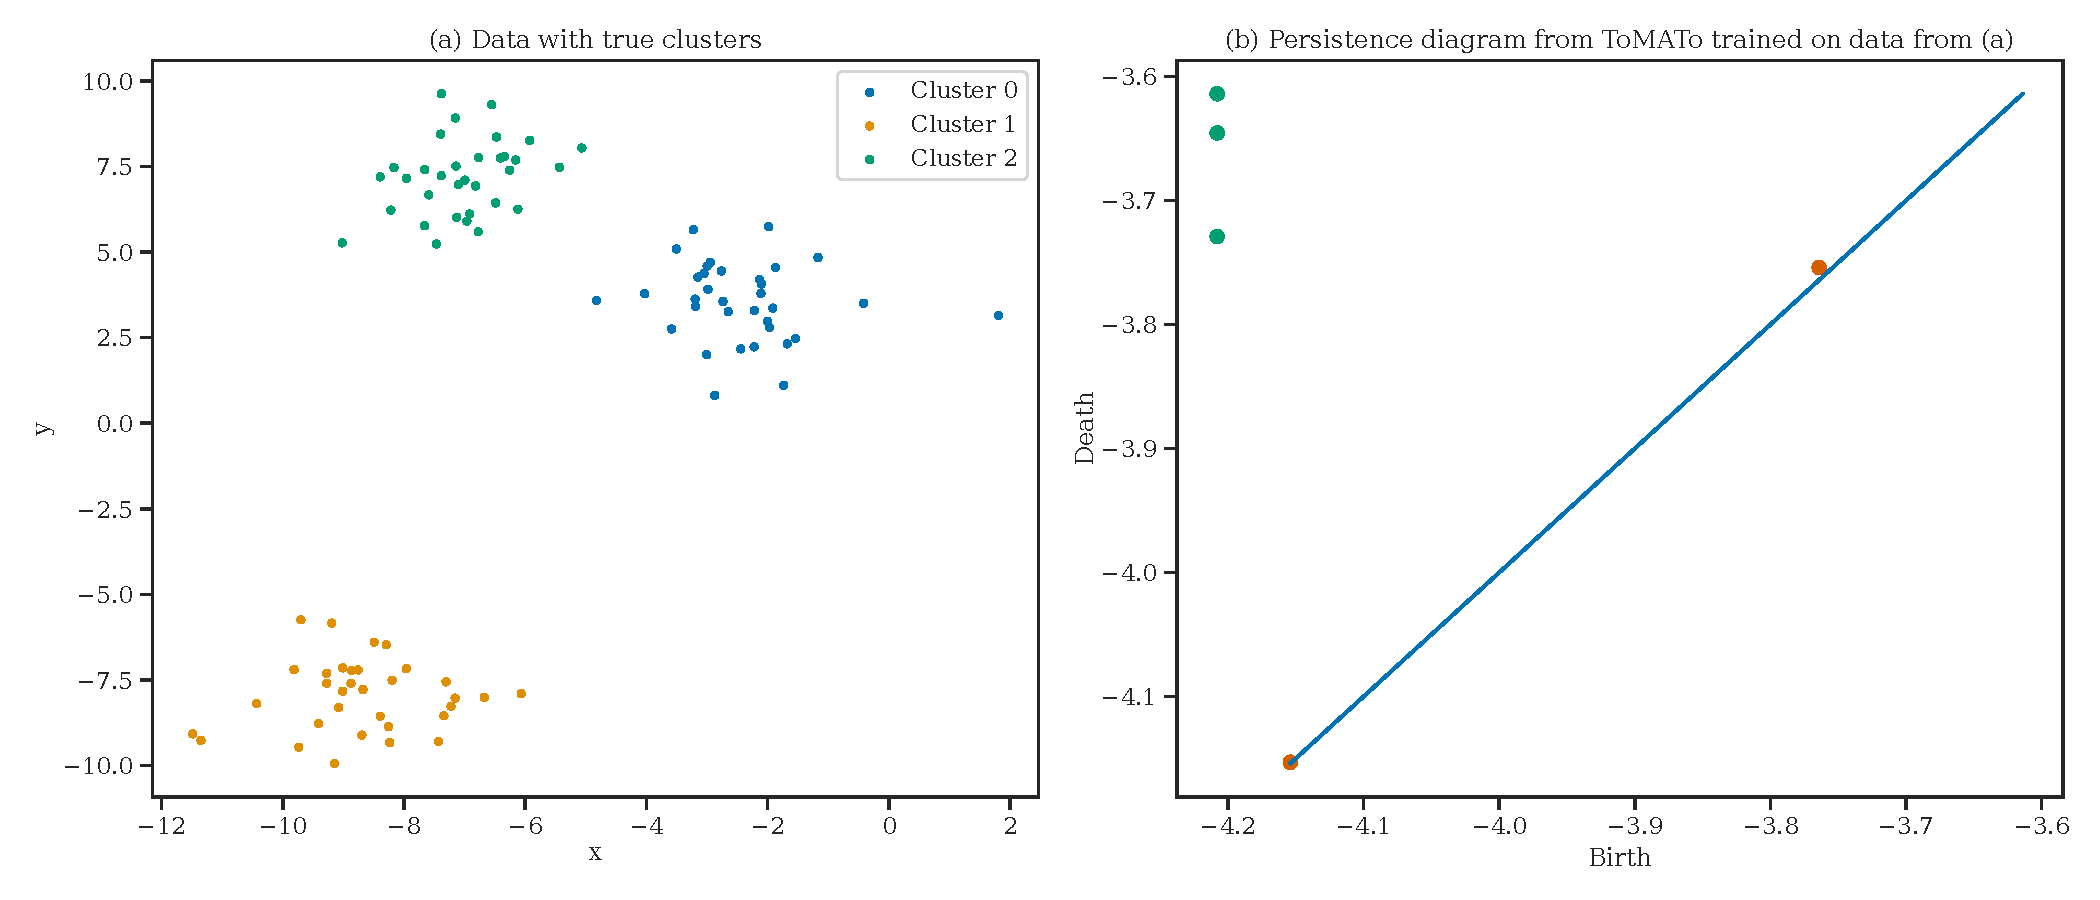
\includegraphics[width=\textwidth]{thesis/figures/k-tomato-clustering-2d-example.pdf}
    \caption{Example of clustering using ToMATo on a 2-dimensional data set with 3 clusters. The persistence diagram in (b) shows the three prominent clusters (green dots).}
    \label{fig:k-tomato-clustering-2d-example}
\end{figure}

What is great about ToMATo is that it gives us a way to determine the numbers of clusters automatically (e.g. using some heuristic on the first persistence diagram to determine $\hat{\tau}$). In addition to this, ToMATo works with any metric, as long as we can create a neighbourhood graph (e.g. using Euclidean distance or similar metrics).

\subsubsection{Comparison of clustering algorithms}
\label{sec:comparison-of-clustering-algorithms}
In \cref{sec:clustering-algorithms}, we describe several algorithms for clustering data. We tabularize the strengths and weaknesses for each algorithm in \cref{table:clustering-algorithms-comparison}. Even though some algorithms might tick off more properties than others, it does not mean that it is a perfect algorithm for all types of data sets. In particular, we have to perform cluster validation to evaluate the results from various cluster algorithms to figure out what algorithm works the best. We explain how to validate results from cluster algorithms in \cref{sec:cluster-validation}.
\begin{table}[H]
    \centering
    \begin{tabular}{@{}lcccccccc@{}}
    \toprule
        & \multicolumn{8}{c}{Algorithm} \\ \cmidrule(l){2-9} 
        \multicolumn{1}{c}{Property} & \multicolumn{1}{l}{\rot{k-means}} & \multicolumn{1}{l}{\rot{MB k-means}} & \multicolumn{1}{l}{\rot{k-medoids}} & \multicolumn{1}{l}{\rot{GMMs}} & \multicolumn{1}{l}{\rot{Hierarchical}} & \multicolumn{1}{l}{\rot{Spectral}} & \multicolumn{1}{l}{\rot{HDBSCAN}} & \multicolumn{1}{l}{\rot{ToMATo}} \\ \midrule
        \trcolor Practical for large data sets & \xmark & \xmark & & \xmark & \xmark & & \xmark & \xmark \\
        Determining the number of clusters automatically & & & & & \xmark & & \xmark & \xmark \\
        \trcolor Cluster centroids as data points & & & \xmark & & & & & \\
        Different clusters shapes & & & & \xmark & \xmark & & \xmark & \xmark \\
        \trcolor Hierarchical clustering & & & & & \xmark & & \xmark & \\
        Robust against nosy data sets & & & \xmark & & & \xmark & \xmark & \xmark \\
        \trcolor Can identify noisy/anomalous data points & & & & & & & \xmark & \xmark \\
        User-defined distance metric & & & \xmark & & \xmark & \xmark & \xmark & \xmark \\ \bottomrule
    \end{tabular}
    \caption{Comparison of various properties for each clustering algorithm we describe in \cref{sec:clustering-algorithms}.}
    \label{table:clustering-algorithms-comparison}
\end{table}

\subsection{Cluster validation}
\label{sec:cluster-validation}
After we use clustering algorithms to perform clustering, we evaluate the result to find the best set of hyperparameters and/or clustering algorithm. This raises the question: Which clustering algorithm performs the best on our data? Thankfully, there exist a handful of various methods to tackle this task. In particular, we differentiate between \textit{internal} and \textit{external cluster validation algorithms}. Internal cluster validation algorithms assess the performance of the clustering using statistics of the data, without knowing the true labels at hand. External cluster validation algorithms, on the other hand, use the knowledge of the true labels. In this thesis, we only use internal cluster validation algorithms, as we are mostly working with data where we do not know the labels beforehand. Recall that, in most clustering algorithms, we want the average distance between any two data points in the same cluster to be as small as possible (compactness); and the average distance between any two data points from different clusters to be as large as possible (separation). Internal cluster validation algorithms usually reflect compactness or separation of clusterings. In the next sub-subsections, we explain some common choices of internal cluster validation algorithms and discuss their strengths and weaknesses. Furthermore, we will use the cluster validation methods we explain below when we analyze word embeddings (\cref{sec:word-embeddings}) in \cref{chap:analysis-of-word-embeddings}.

\subsubsection{Silhouette Coefficient}
\label{sec:silhouette-coefficient}
The \textit{Silhouette Coefficient} is an internal cluster validation method that measures the goodness of clusterings \cite[p. 87]{Kaufman1990}. In particular, the Silhouette Coefficient measures how similar data points are to their own cluster (compactness) when we compare to data points from other clusters (separation). The Silhouette Coefficient ranges from -1 to 1, where the best value is 1 and the worst value is -1. Values near 0 indicate that we have overlapping clusters (i.e. low separation). We base this sub-subsection on \cite[p. 87]{Kaufman1990}.

For any data point $x_i$ in the cluster $C_i$, we compute the mean compactness $a(i)$ as the average distance $d(i, j)$ between data point $i$ and all other data points in $C_i$, i.e. $j \in C_i, i \neq j$. More formally, we define the mean compactness $a(i)$ as
\begin{align}
    a(i) = \frac{1}{|C_i| - 1} \sumlim{j \in C_i, i \neq j}{}{d(i, j)},
    \label{eqn:silhouette-coef-a}
\end{align}
where $|C_i|$ is the number of data points in cluster $C_i$. Smaller values of $a(i)$ indicate better compactness of clusters, and thus, better cluster assignments. Following, for any data point $x_i$ in the cluster $C_i$, we compute the mean separation $b(i)$ as the smallest distance from $i$ to any other cluster in which $i$ does not belong. The mean separation $b(i)$ is defined as
\begin{align}
    b(i) = \min_{k \neq i} \frac{1}{|C_k|} \sumlim{j \in C_k}{}{d(i, j)}.
    \label{eqn:silhouette-coef-b}
\end{align}
Large values of $b(i)$ indicate that the clusters have good separation and that data points in $C_i$ are a good fit. Now, using the definitions of compactness and separation, we define the \textit{silhouette} of data point $i$ as
\begin{align}
    s(i) = \begin{cases}
        \frac{b(i) - a(i)}{\max \enclp{a(i), b(i)}} & \mbox{if } |C_i| > 1 \\
        0 & \mbox{if } |C_i| = 1
    \end{cases}.
\end{align}
Taking the average of all silhouettes $s(i)$, we define the \textit{mean Silhouette Coefficient} as
\begin{align}
    SC = \frac{1}{n} \sumlim{i=1}{n}{s(i)},
    \label{eqn:silhouette-coef}
\end{align}
where $n$ is the number of data points in our data (e.g. $n$-dimensional data $X$).

The main advantages of the mean Silhouette Coefficient are that it is simple, fast to compute and has a defined range from -1 to 1. The mean Silhouette Coefficient struggles with overlapping clusters (where $SC \approx 0$).

\subsubsection{Davies-Bouldin Index}
\label{sec:davies-bouldin-index}
The \textit{Davies-Bouldin Index} (DBI) is an internal cluster validation method for evaluating results of clustering algorithms \cite{DaviesBouldin1979}. Similar to the Silhouette Coefficient, DBI measures the compactness and separation of clusters to measure the goodness of fit. We base this sub-subsection on \cite{DaviesBouldin1979}.

To measure the compactness of clusters, DBI introduces the notion of \textit{scatter within a cluster}, which we denote $S_i$. We compute $S_i$ by taking the mean of the sum of the distances to the cluster centroid of a particular data point $i$. More formally, we define $S_i$ as
\begin{align}
    S_i = \enclp{ \frac{1}{|C_i|} \sumlim{x_j \in C_i}{} |x_j - \Tilde{C_i}|^p}^{1/p},
    \label{eqn:dbi-s}
\end{align}
where $C_i$ is the cluster we associate to data point $i$, $|C_i|$ is the number of data points in cluster $C_i$, $\Tilde{C_i}$ is the centroid of cluster $C_i$ and $p$ denotes the power of the $L^p$ distance. A common choice is to set $p=2$, leading to Euclidean distances. A low value of $S_i$ indicates that the compactness of cluster $C_i$ is good. To compute the separation of clusters, DBI computes separation between clusters $C_i$ and $C_j$ by taking the distance between cluster centroids $\Tilde{C_i}$ and $\Tilde{C_j}$. We define the cluster separation $M_{i, j}$ as
\begin{align}
    M_{i, j} = ||\Tilde{C_i} - \Tilde{C_j}||_p,
    \label{eqn:dbi-m}
\end{align}
where $p$ denotes the power of the $L^p$ distance. High values of $M_{i, j}$ indicate that we separate the clusters well. Combining the notion of cluster compactness $S_i$ and separation $M_{i, j}$, we define the measure of cluster goodness $R_{i, j}$ as
\begin{align}
    R_{i, j} = \frac{S_i + S_j}{M_{i, j}}.
    \label{eqn:dbi-r}
\end{align}
To create a clustering measure that is symmetric and non-negative, we define $R_{i, j}$ as such. Low values of $R_{i, j}$ indicate that we have compact clusters with high separation. For a particular cluster $C_i$, DBI measures $R_{i, j}$ for all other clusters $C_j$, $j \neq i$, and uses the largest value of $R_{i, j}$, i.e. the worst-case scenario, to compute the index. More formally, we define DBI as
\begin{align}
    DBI = \frac{1}{n} \sumlim{i=1}{n} \max_{j \neq i} R_{i, j},
    \label{eqn:dbi}
\end{align}
where $n$ is the number of data points in our data (e.g. $n$-dimensional data $X$). The main advantage of DBI is the fact that is fast to compute and has non-negative values. Since DBI does not have any upper bound, it is more difficult to interpret the values, when we for instance compare it to Silhouette Coefficient.

\subsubsection{Caliński-Harabasz Index}
\label{sec:calinski-harabasz-index}
The \textit{Caliński-Harabasz Index} (CHI) is an internal cluster validation method for evaluating clustering algorithms \cite{CalinskiHarabasz1974}. CHI measures compactness and separation of clusters to measure the goodness of fit of a particular clustering. We base this sub-subsection on \cite{CalinskiHarabasz1974}.

To measure the compactness of a clustering, CHI computes the \textit{sum-of-squares within cluster} (SSW) as
\begin{align}
    SSW = \sumlim{i=1}{n} ||x_i - \Tilde{C_i}||^2,
    \label{eqn:chi-ssw}
\end{align}
where $n$ is the number of data points in our data, $x_i$ is the $i$th data point and $\Tilde{C_i}$ is the centroid of the cluster we associate to $x_i$. Small values of SSW indicate that we have compactly clustered data points. To measure the separation of clusters, CHI computes the \textit{sum-of-squares between clusters} (SSB) as
\begin{align}
    SSB = \sumlim{j=1}{k} |C_j| \cdot ||\Tilde{C_i} - \Bar{X}||^2,
    \label{eqn:chi-ssb}
\end{align}
where $k$ is the number of clusters, $|C_j|$ is the number of data points in cluster $C_j$ and $\overline{X}$ is the centre of all data points (i.e. mean). Large values of SSB indicate that we have a good separation of the clusters. Finally, we compute the CHI by multiplying the ratio of SSB to SSW with a weight depending on $n$ and $k$. More formally, the CHI is defined as
\begin{align}
    CHI = \frac{SSB}{SSW} \times \frac{n - k}{k - 1}.
    \label{eqn:chi}
\end{align}
Since we define CHI as the ratio between SSB and SSW, large values indicate better clustering. The main advantage of CHI is that it is fast to compute. Similar to Davies-Boundin Index, CHI is harder to interpret than Silhouette Coefficient for example, since the values do not have any upper limit.

\subsection{Dimensionality reduction methods}
\label{sec:dimensionality-reduction-methods}
Working with data in high dimensions can be a difficult task. Imagine that we have gathered some data, containing several features, and we would like to deepen our understanding of it. One approach we could do would be to visualize each feature by plotting them against each other, looking for bivariate relationships. Unfortunately, this is a rather cumbersome task and is hard to employ once a certain number of features is met (e.g. 10 features). Thankfully, \textit{dimensionality reduction methods} can help us to reduce the dimensionality of data into some lower dimension, preserving relevant properties of the original data in the process. A typical application of dimensionality reduction methods is to lower the dimensionality to 2 or 3 such that we can visualize the data at ease. We introduce two dimensionality reduction methods and explain how they work. In both sub-subsections below, we assume that we have some data $X \in \R^{n \times d}$ and that we want to reduce the dimensionality to some chosen hyperparameter $k$. Furthermore, we will use the dimensionality reduction methods which we explain below when we analyse clustering of word embeddings (\cref{sec:word-embeddings}) in \cref{chap:analysis-of-word-embeddings} and prediction of polysemous words in \cref{sec:analysis-of-embeddings-supervised-polysemy-prediction}.

\subsubsection{Principal Component Analysis}
\label{sec:pca}
\textit{Principal Component Analysis} (PCA) is one of the most common dimensionality reduction methods \cite{Jolliffe2002}. PCA performs a linear mapping of the original data $X \in \R^{n \times d}$ to a (possibly) lower-dimensional space $Y \in \R^{n \times k}$ ($k \leq d$) such that the variance is maximal in $Y$. We typically select $k$ to be a relatively low value, e.g. 2 or 3, if we would like to visualize it using plots. Another common value for $k$ is to set it such that a specific variance threshold is met, e.g. explaining 90\% of the variance of the data. We refer to \cite{Jolliffe2002} when explaining PCA.

The PCA algorithm consists of several steps, and following, we explain each step. First, compute the mean of $X$, which we denote $\overline{X} = \frac{1}{n} \sumlim{i=1}{n} x_i$, and subtract it from $X$, i.e. $X' = X - \overline{X} = \enclc{x'_1, x'_2, \ldots, x'_n}$. Next, we compute the covariance matrix of $X'$, which we denote $C \in \R^{d \times d}$, and we compute the corresponding eigenvectors and eigenvalues of $C$, which we denote $C_\text{eig} = \enclc{c_1, c_2, \ldots, c_d}$. Furthermore, we sort the eigenvectors $C_\text{eig}$ by its corresponding eigenvalues in a descending manner. By doing so, we get a set of eigenvectors such that the first eigenvector corresponds with the largest value, the second eigenvector corresponds with the second largest value and so forth. We denote this set of eigenvectors as $C'_\text{eig} = \enclc{c'_1, c'_2, \ldots, c'_d}$. We then pick the $k$ first eigenvectors of $C'_\text{eig}$ and project the data onto them, essentially performing a \textit{change of basis}. In addition to this, we add the mean of $X$ to complete the reconstruction. We define the reconstruction of PCA as
\begin{align}
    Y = X' \trans{\begin{pmatrix}
    c'_1 & c'_2 & \ldots & c'_k
    \end{pmatrix}} + \overline{X},
    \label{eqn:pca-projection}
\end{align}
where $Y = \enclc{y_1, y_2, \ldots, y_n}$ represents the original data $X$ in (a possibly) lower dimension $k$, such that we maximize the variance of the vectors of $X$. We refer the vectors $\enclc{y_1, y_2, \ldots, y_n}$ as the principal components (PC) of $X$, where PC1 is $y_1$, PC2 is $y_2$ and so forth. Finally, we show an example where we apply PCA to some 2-dimensional data in \cref{fig:pca-2d-example}, where we see that PCA essentially rotates the data, maximizing the variance in the PC axes.
\begin{figure}[H]
    \centering
    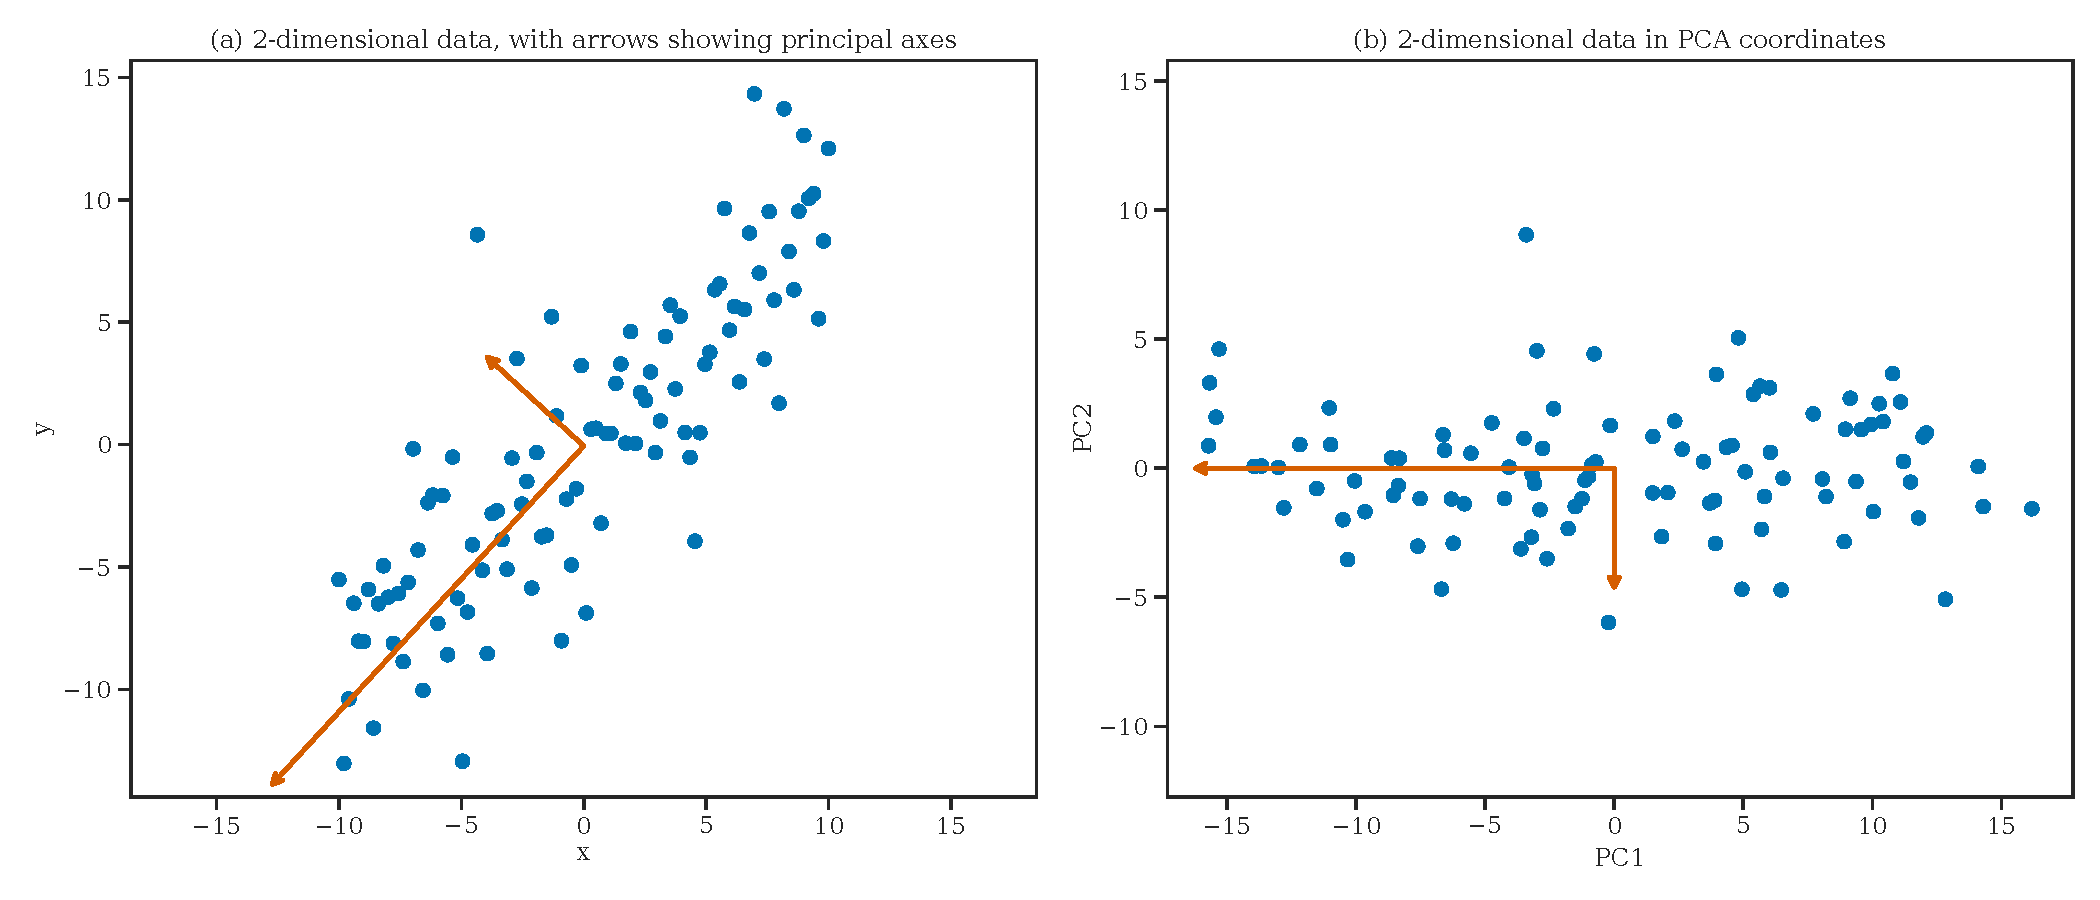
\includegraphics[width=\textwidth]{thesis/figures/pca-2d-example.pdf}
    \caption{PCA applied to 2-dimensional data, showing the principal axes by the arrows.}
    \label{fig:pca-2d-example}
\end{figure}

\subsubsection{Uniform Manifold Approximation and Projection}
\label{sec:umap}
\textit{Uniform Manifold Approximation and Projection} (UMAP) is a dimensionality reduction algorithm that, among other things, uses ideas from topological data analysis \cite{2018arXivUMAP}. In particular, UMAP uses a fuzzy version of simplicial complexes (see \cref{sec:simplicial-complex} for the definition of a simplicial complex) to create a graph representing the topological structure of the data in its original (high) dimension. To explain how UMAP works, we use the example from the "How UMAP Works" documentation page \cite{how-umap-works-2018}.

Imagine that we have some data from a noisy sine, $X = \enclc{x_1, x_2, \ldots, x_n} \in \R^{n \times d}$, as we see in \cref{fig:how_umap_works_raw_data}.
\begin{figure}[H]
    \centering
    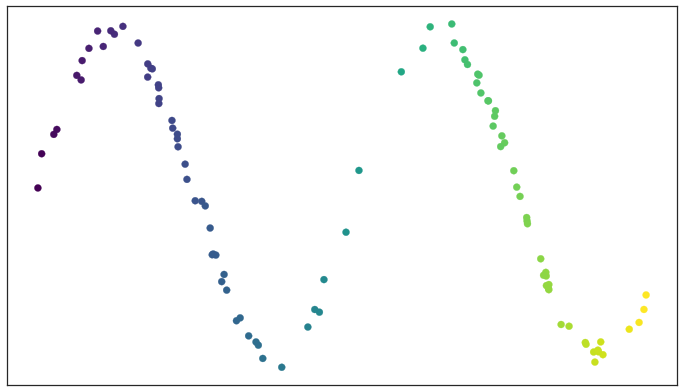
\includegraphics[width=0.8\textwidth]{thesis/figures/how_umap_works_raw_data.png}
    \caption{A noisy sine wave. The figure is from \cite{how-umap-works-2018}.}
    \label{fig:how_umap_works_raw_data}
\end{figure}

We would like to capture the topological structure of $X$, and we do so by creating a simplicial complex built on $X$, as we see in \cref{fig:how_umap_works_basic_graph}.
\begin{figure}[H]
    \centering
    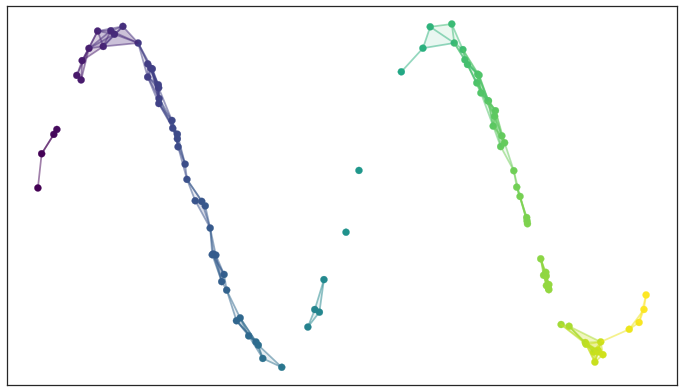
\includegraphics[width=0.8\textwidth]{thesis/figures/how_umap_works_basic_graph.png}
    \caption{A simplicial complex built on a noisy sine wave. The figure is from \cite{how-umap-works-2018}.}
    \label{fig:how_umap_works_basic_graph}
\end{figure}
We would like to capture the topological structure of all data points in $X$ and want a graph connecting all points. By using simplicial complexes, however, we see in \cref{fig:how_umap_works_basic_graph} that problems can occur, namely that not all data points have edges between them, which again disconnects the simplicial complex. This particular problem can occur when we have a too-small $\epsilon$ radius around each data point. In real-world data, the data points are typically not laying on a uniform distribution. Moreover, selecting a perfect $\epsilon$ to create a suitable simplicial complex is hard. The authors of UMAP overcome these problems by creating fuzzy open sets around each data point to create local connectivity in the graph, as we see in \cref{fig:how_umap_works_umap_open_cover}.
\begin{figure}[H]
    \centering
    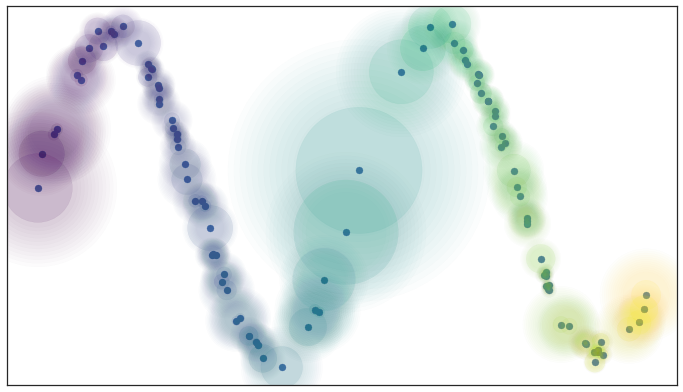
\includegraphics[width=0.8\textwidth]{thesis/figures/how_umap_works_umap_open_cover.png}
    \caption{Fuzzy open sets around each data point of a noisy sine wave to create local connectivity. The figure is from \cite{how-umap-works-2018}.}
    \label{fig:how_umap_works_umap_open_cover}
\end{figure}
To create the fuzzy open sets, we compute the distance to the nearest neighbour of each data point and the level of \textit{fuzziness} decreases in terms of the distance beyond it, starting from 1 decreasing to 0. If a data point has a fuzziness level greater than zero, then we create an edge between the two data points, with weight equal to the fuzziness level. Furthermore, we interpret the fuzziness level as the probability of the edge existing. We illustrate the connected graph in \cref{fig:how_umap_works_raw_graph}.

\begin{figure}[H]
    \centering
    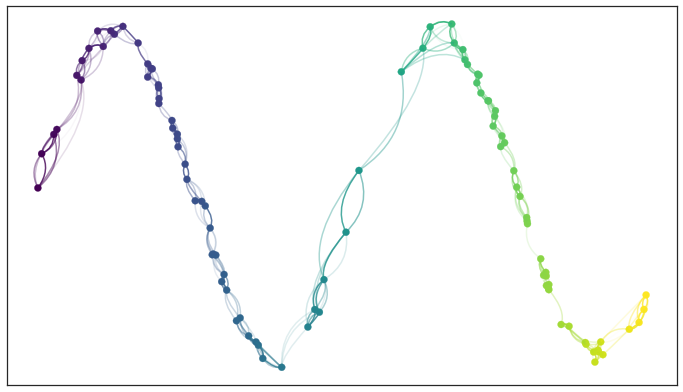
\includegraphics[width=0.8\textwidth]{thesis/figures/how_umap_works_raw_graph.png}
    \caption{A connected graph where nodes are data points and the edges between them have the fuzziness levels as weights. The figure is from \cite{how-umap-works-2018}.}
    \label{fig:how_umap_works_raw_graph}
\end{figure}
To finalize the connected graph from \cref{fig:how_umap_works_raw_graph}, we convert the edges between any two data points into a single edge. We do this because we want the distance between two data points $a$ and $b$ to be the same; currently, it depends locally on the distance to the nearest neighbour, as the fuzziness level decreases beyond it. To merge the edges between any two data points $a$ and $b$, we compute the combined weight by taking the union between them $w(a) + w(b) - w(a)w(b)$. We use the newly combined weight as the weight of the single edge between $a$ and $b$. If we apply this process, unioning edges together, we end up with a fuzzy simplicial complex. We show an example of a fuzzy simplicial complex in \cref{fig:how_umap_works_umap_graph}.
\begin{figure}[H]
    \centering
    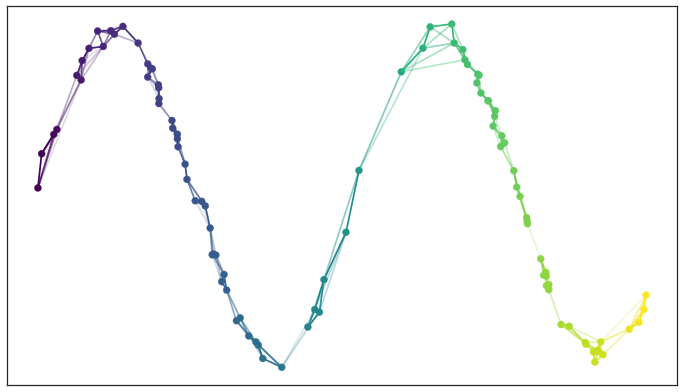
\includegraphics[width=0.8\textwidth]{thesis/figures/how_umap_works_umap_graph.png}
    \caption{A fuzzy simplicial complex of some sine wave data. The figure is from \cite{how-umap-works-2018}.}
    \label{fig:how_umap_works_umap_graph}
\end{figure}
Now, using the fuzzy simplicial complex of \cref{fig:how_umap_works_umap_graph}, we have a topological representation of $X$, capturing the topology of the manifold. We denote the set of all possible 1-simplices (i.e. edges) as $E$. To compute the weight of a 1-simplex (i.e. edge) $e$, we use $w_h(e)$ in the high dimensional case. To get a good low dimensional representation of the high dimensional fuzzy simplicial complex, we initialize a low dimensional fuzzy simplicial complex. We denote the weights of the low dimensional fuzzy simplicial complex as $w_l(e)$ for edge $e$. To determine the weights $w_l(e)$, we employ an iterative process where we optimize a loss function $L$ in a gradient descent fashion (see \cref{sec:ann-loss-functions,sec:ann-optimizers} for more information regarding loss functions and the gradient descent optimizer). Since we interpret the weights of the 1-simplices of $E$ as probabilities of the edge existing (i.e. Bernoulli variables), the authors of UMAP uses cross-entropy (see \cref{eqn:binary-cross-entropy}) as the loss function. More formally, we define the loss function $L$ as
\begin{align}
    L = \sumlim{e \in E}{} \undertext{w_h(e) \log \enclp{\frac{w_h(e)}{w_l(e)}}}{Attractive force} + \undertext{(1 - w_h(e)) \log \enclp{\frac{1 - w_h(e)}{1 - w_l(e)}}}{Repulsive force}.
    \label{eqn:umap-loss-function}
\end{align}

In the first term of \cref{eqn:umap-loss-function}, we have an attractive force between the data points which $e$ spans, pulling them together; when $w_l(e)$ is large, the distance (i.e. weight) between any two data points becomes small. In the second term of \cref{eqn:umap-loss-function}, there is an opposite, repulsive force between the data points which $e$ spans, repelling them apart; when $w_h(e)$ is small (i.e. distance in high dimensional space), $w_l(e)$ becomes small since we want to minimize the term. The process of pulling and repelling the weights makes the low dimensional representation of the data settle into a balanced state, such that it represents the high dimensional topological structure of the original data in a fairly accurate way. In practice, the UMAP algorithm uses several different tricks to optimize it, but we leave out the technical details here. We kindly refer the reader to \cite{2018arXivUMAP} for more details. Finally, we show an example where we compute a 2-dimensional UMAP embedding of the Iris data set \cite{Anderson1936,Fisher1936} in \cref{fig:umap-2d-example}, where we see that UMAP can separate the classes in the Iris data set quite nicely, particularly for the \textit{setosa} class.
\begin{figure}[H]
    \centering
    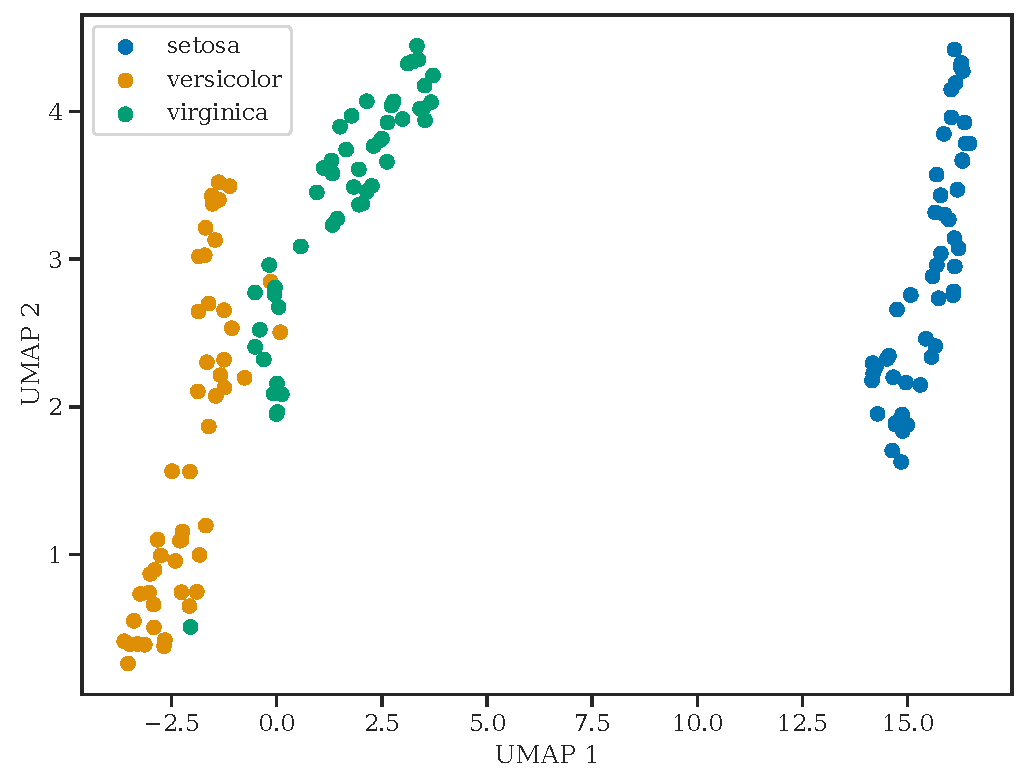
\includegraphics[width=0.8\textwidth]{thesis/figures/umap-2d-example.pdf}
    \caption{2-dimensional UMAP embedding of the Iris data set \cite{Anderson1936,Fisher1936}.}
    \label{fig:umap-2d-example}
\end{figure}

\subsection{Artificial neural networks}
\label{sec:artificial-neural-networks}
In this subsection we explain \textit{artificial neural networks} (ANN). In particular, we focus on \textit{multilayered neural networks} (MLNN). We base this subsection on \cite[Chapter 1]{Aggarwal18} and \cite{rong2016word2vec}. Furthermore, we will use the notion of artificial neural networks when we explain the word2vec model in \cref{sec:word2vec-as-an-ann}.

An \textit{artificial neuron} (or \textit{unit}) is a function which receives one or more inputs and a \textit{bias}, and then sums them to produce an output. We illustrate an example of an artificial neuron in \cref{fig:artificial_neuron}, where $\left\{ x_1, \ldots, x_K \right\}$ are the input values, $b$ is the bias, $\left\{ w_1, \ldots, w_K \right\}$ are the weights and $y$ is a scalar output. We denote $f$ as the \textit{activation function}.
\begin{figure}[H]
    \centering
    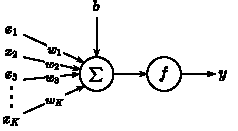
\includegraphics[width=0.5\textwidth]{thesis/figures/artificial-neuron_cropped.pdf}
    \caption{An artificial neuron that takes in a $K$-dimensional input $x$ and bias $b$ to produce some output $y$.}
    \label{fig:artificial_neuron}
\end{figure}

We produce the output of a single unit by applying an activation function $f$ to the input $u$. More formally, we define the output of a single unit as
\begin{align}
    y = f(u),
\end{align}
where $u$ is the input of the neuron. We define $u$ as
\begin{align}
    u = b + \sumlim{i=1}{K} w_i x_i,
\end{align}
which is the weighted sum of the input values $\left\{ x_1, \ldots, x_K \right\}$ plus the bias term, with $\left\{ w_1, \ldots, w_K \right\}$ as weights.

The bias term acts as an intercept value to make the model more general and is usually set to +1. For some models (e.g. word2vec, which we introduce as an ANN in \cref{sec:word2vec-as-an-ann}), we exclude the bias term for the units in the neural network, i.e. we leave $b$ to be zero.

The choice of activation function $f$ is typically a non-linear function. Artificial neural networks use different activation functions such as ReLU, sigmoid or tanh to learn non-linear relationships in the data. We come back to the concept of activation functions in \cref{sec:ann-activation-functions}.

\newcommand{\layer}[2]{\left\{ {#1}_{#2} \right\}}

A \textit{layer} $\layer{z}{j} = \left\{ z_1, z_2, \ldots, z_K \right\}$ of an artificial neural network is a collection of artificial neurons (unit). We define the layer $\layer{z}{j}$ using an $N \times K$-dimensional weight matrix $W$, a $N$-dimensional bias vector $b$ and an activation function $f$. More formally, we define a layer $\layer{z}{j}$ as
\begin{align}
    \layer{z}{j} = f \left( W \cdot x + b \right),
    \label{eqn:artificial_layer}
\end{align}
where $x$ is a $K$-dimensional input vector. In the following sub-subsections, we explain the different types of layers in the ANN, namely the input, hidden and output layers.

\subsubsection{Input layer}
\label{sec:ann-input-layer}
The first layer in the ANN is the \textit{input layer} $\layer{x}{k} = \left\{ x_1, x_2, \ldots, x_K \right\}$. It is responsible for taking in input and passing it to the proceeding layer in the network. We illustrate the input layer in \cref{fig:input_layer_ann}, where we see that each input value $x_i$ gets its own node.
\begin{figure}[H]
    \centering
    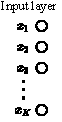
\includegraphics[height=5cm]{thesis/figures/artificial-neural-network-input-layer_cropped.pdf}
    \caption{Input layer in the ANN for a $K$-dimensional vector $x$.}
    \label{fig:input_layer_ann}
\end{figure}
Following, we define the input layer more formally using \cref{eqn:artificial_layer} in \cref{eqn:input_layer_ann}. We see that the input layer does not perform any changes to the incoming data and acts as a way for feeding data into the neural network. More formally, we define the input layer $\layer{x}{k}$ as
\begin{align}
    \label{eqn:input_layer_ann}
    \layer{x}{k}
    &= f_{\layer{x}{k}}(W_{\layer{x}{k}} \cdot x) \\
    &= id(I_K \cdot x) \notag \\ 
    &= I_K \cdot x \notag \\
    &= x, \notag
\end{align}
where the weight matrix $W_{\layer{x}{k}}$ is the identity matrix $I_K$, we have no bias (i.e. bias equal to zero vector) and the activation function $f_{\layer{x}{k}}$ is the identity function $id(x)=x$. In the following sub-subsection, we look at the next layer in the neural network, namely the hidden layer.

\subsubsection{Hidden layer}
\label{sec:ann-hidden-layer}
The \textit{hidden layer} is the second layer in the ANN $\layer{h}{i} = \left\{ h_1, h_2, \ldots, h_N \right\}$, and we most commonly connect it to the input layer. We note that we can, however, have multiple hidden layers in the ANN by connecting them to each other (making the neural network \textit{deeper}). For illustration purposes, we assume that we only have one hidden layer in our neural network. We illustrate an example of a hidden layer in \cref{fig:hidden_layer_ann}, where we observe that we connect every unit in the input layer to the units in the hidden layer. We illustrate the connections by the lines. This is what we call \textit{fully connected layers}, meaning that we connect every unit to each other.

\begin{figure}[H]
    \centering
    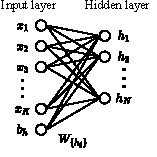
\includegraphics[height=6cm]{thesis/figures/artificial-neural-network-input-hidden-layer_cropped.pdf}
    \caption{Input to hidden layer in the ANN for a $K$-dimensional vector $x$, $N\times K$ dimensional weight matrix $\left\{ W_{h_i} \right\}$ and a $N$-dimensional hidden layer $h$.}
    \label{fig:hidden_layer_ann}
\end{figure}
We formalize the description of the hidden layer by defining it as
\begin{align}
    \label{eqn:hidden-layer-ann}
    \layer{h}{i} &= f_{\layer{h}{i}}(W_{\layer{h}{i}} \cdot \layer{x}{k} + b_h),
\end{align}
where $f_{\layer{h}{i}}$ is a user-specified activation function, $W_{\layer{h}{i}}$ is an $N \times K$-dimensional weight matrix and $b_h$ is an $N$-dimensional bias vector. The hidden layer tries to learn a \textit{latent} (i.e hidden) representation of the input data $x$. We explain how the neural network learns the latent representation when introducing optimizers in \cref{sec:ann-optimizers}. Assuming that we have some $N$-dimensional latent representation of the data, we would like to connect it to the final layer in the neural network, the output layer, which we explain next.

\subsubsection{Output layer}
\label{sec:ann-output-layer}
The last layer in the ANN is the \textit{output layer} $\layer{y}{j} = \left\{ y_1, y_2, \ldots, y_M \right\}$, which we connect to the last hidden layer of the network. Similar to the hidden layer, we connect each unit in the last hidden layer to each unit in the output layer. We illustrate an example of this in \cref{fig:mlnn-one-hidden}, where we see a complete, multilayered neural network (MLNN).
\begin{figure}[H]
    \centering
    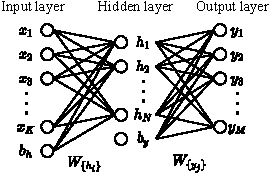
\includegraphics[width=0.6\textwidth]{thesis/figures/artificial-neural-network_cropped.pdf}
    \caption{Multilayered neural network with one input, hidden and output layer.}
    \label{fig:mlnn-one-hidden}
\end{figure}

Following, we define the output layer $\layer{y}{j}$ using a $M \times N$ weight matrix $W_{\layer{y}{j}}$, an $M$-dimensional bias vector $b_y$ and an activation function $f_{\layer{y}{j}}$. More formally, we define the output layer $\layer{y}{j}$ as
\begin{align}
    \label{eqn:output-layer-ann}
    \layer{y}{j} &= f_{\layer{y}{j}}(W_{\layer{y}{j}} \cdot \layer{h}{i} + b_y).
\end{align}

We have now covered the different layers in an MLNN, but have yet to cover the different choices of activation function $f$ in the neural network and how the MLNN learns. In the following sub-subsections, we look at choices of activation and loss functions, as well as optimizers for learning in the network.

\subsubsection{Activation functions}
\label{sec:ann-activation-functions}
The input data we use to feed into an ANN can contain complex patterns and have non-linear relationships. To learn such patterns and relationships, we apply an activation function to each layer before the result is sent to the proceeding layer. There are several choices of activation functions and following, we explain some of the most common ones.

The simplest type of activation is the identity function, which we define as
\begin{align}
    \label{eqn:identity-function}
    f(x) = x.
\end{align}
We commonly use the identity function when we want to pass on the values from one layer to another without modifying the value itself, as we use in the input layer from \cref{sec:ann-input-layer}. Other choices of activation functions include \textit{sigmoid}, \textit{tanh}, \textit{Rectified Linear Unit} (ReLU) and \textit{softmax}. We visualize activation functions in \cref{fig:activation-functions} and define them formally below as
\begin{align}
    \label{eqn:sigmoid-function}
    f(x) &= \frac{1}{1 + \exp{ \left( -x \right) }} \thickspace \text{(sigmoid function)}, \\
    \label{eqn:tanh-function}
    f(x) &= \frac{\exp{ \left( 2x \right) } - 1}{\exp{ \left( 2x \right) } + 1} \thickspace \text{(tanh function)}, \\
    \label{eqn:relu-function}
    f(x) &= \max{\left\{ x, 0 \right\}} \thickspace \text{(ReLU function)}, \intertext{and}
    \label{eqn:softmax-function}
    f(x_i) &= \frac{\exp \left( x_i \right)}{\sumlim{j=1}{K} \exp \left( x_j \right)} \thickspace \text{, $i \in \left\{ 1, \ldots, K \right\}$ (softmax function)},
\end{align}
where $K$ is the number of output values for the softmax layer.

\begin{figure}[H]
    \centering
    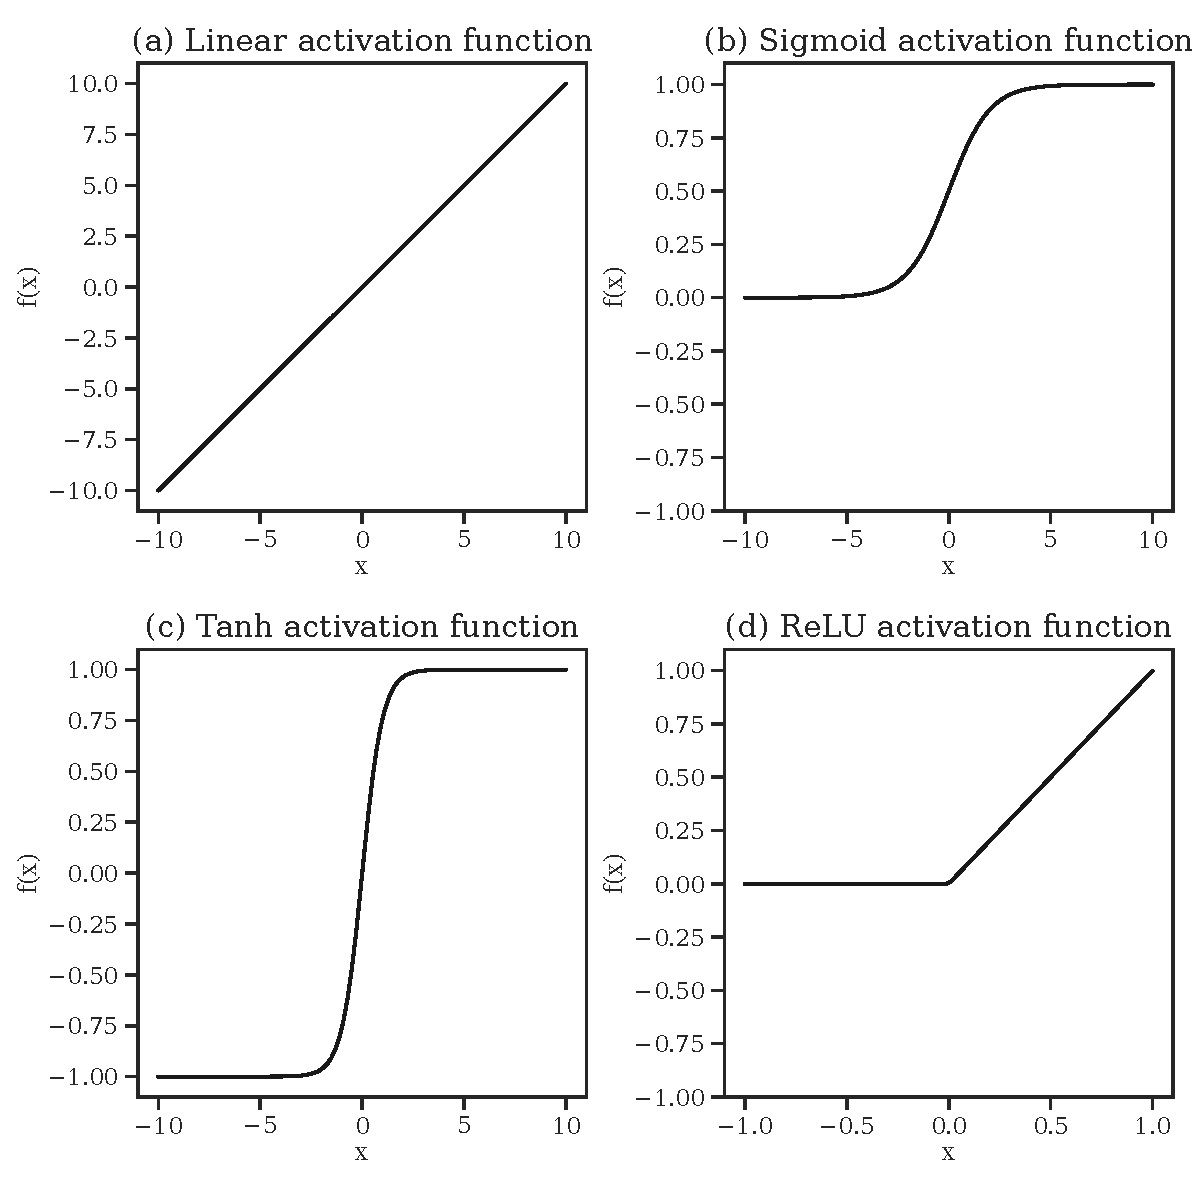
\includegraphics[width=0.8\textwidth]{thesis/figures/common-activation-functions.pdf}
    \caption{Four plots of various activation functions showing how they respond to different values of $x$.}
    \label{fig:activation-functions}
\end{figure}

The sigmoid and tanh activation functions were typically used in the early development of neural networks. The sigmoid activation function maps a value to a value in $(0, 1)$ and is particularly useful since it creates a probabilistic output. The tanh activation function has a similar shape to the sigmoid activation function and maps values to values in $[-1, 1]$. We show the relationship between the tanh and sigmoid activation functions as
\begin{align}
    \label{eqn:tanh-sigmoid-relation}
    \text{tanh}(x) = 2 \cdot \text{sigmoid}(2x) - 1,
\end{align}
where we see that the tanh activation function is a rescaled version of the sigmoid activation function.

In more recent years, the ReLU activation function has become more popular, partly due to its computational simplicity. Both the sigmoid and tanh activation function suffers from \textit{vanishing gradients} (i.e. gradients become zero, leading to practically no learning) and we typically use ReLU as a substitute to overcome this problem. This does not mean, however, that we can use the ReLU activation function without problems, as it can "die out" since it is non-differentiable at 0.

Up until now, we have only explained activation functions in the context of a single output value. To perform classification with $K$ outputs, we typically use the softmax activation function, which we define in \cref{eqn:softmax-function}. We interpret the output of the softmax activation function as the probabilities of the $K$ outputs. Next, we look at loss functions in neural networks.

\subsubsection{Loss functions}
\label{sec:ann-loss-functions}
By connecting the different layers in an ANN, we have seen how we use some input data, send it through some hidden layer, and finally, get the predicted output values from the output layer. We denote the predicted output values as $\hat{y}$ and assume that we have the true output values as well, which we denote $y$. The \textit{loss function} measures how much the predicted values $\hat{y}$ deviate from the true values $y$, and as such, the goal is to minimize this value. The output layer can have one or many outputs, and depending on the configuration of the network, the loss function changes as well. We separate the output types of an ANN into two categories, namely the \textit{regression} and \textit{classification} outputs.

In a regression type output, we usually predict some real-value quantity, such as height, weight or distance. For such problems, it is common to use the \textit{mean squared error} (MSE) as the loss function. We calculate the MSE as the mean of the squared differences between the predicted and true values. More formally, we define MSE as
\begin{align}
    \label{eqn:mean-squared-error}
    \text{MSE}(\hat{y}, y) = \frac{1}{N} \sumlim{i=1}{N} {\left( y_i - \hat{y_i} \right)}^2,
\end{align}
where $N$ is the length of $y$ and $\hat{y}$.

For classification type outputs, we want to classify whether or not some input data belongs to two (binary, e.g. on or off, blue or red) or more classes (categorical, e.g. different types of animals). In a binary classification type output, we use the sigmoid activation function in conjunction with the \textit{binary cross-entropy} (BCE) loss function. We define the binary cross-entropy loss function as
\begin{align}
    \label{eqn:binary-cross-entropy}
    \text{BCE}(\hat{y}, y) = -\left( y \cdot \log{\left( \hat{y} \right)} + (1 - y) \cdot \log{\left( 1 - \hat{y} \right)} \right).
\end{align}
As opposed to the binary cross-entropy function, we use the \textit{categorical cross-entropy} (CCE) function to compute the loss for multi-class classification output. We commonly use the softmax activation function in the output layer to create a multi-class probability distribution. Furthermore, we define the CCE loss function as
\begin{align}
    \label{eqn:categorical-cross-entropy}
    \text{CCE}(\hat{y}, y) = -\sumlim{c=1}{C} y_c \cdot \log{\left( \hat{y_c} \right)},
\end{align}
where $C$ is the number of classes in the multi-class classification output. In \cref{eqn:categorical-cross-entropy}, we observe that CCE is simply a generalization of the BCE loss function for multiple classes.

\subsubsection{Optimizers}
\label{sec:ann-optimizers}
In this sub-subsection, we explain how an ANN can effectively make predictions from input data by learning its internal weights. In particular, we explain the gradient descent algorithm and how ANNs exploit it to perform efficient training of its internal parameters.

So far, we have discussed what we call the \textit{forward pass} (or phase). A forward pass is simply the journey of the input data to the output layers where we in each step compute the output values at each layer and local derivatives using the current set of weights. Once we are at the output layer, the forward pass is complete and the \textit{backward pass} commences. Recall that the objective of the neural network is to minimize the loss function. To do so, we compute the derivative of the loss function with respect to the weights in the input layer, using the chain rule from calculus. The derivative of the loss function tells the neural network which direction it should move each weight in to minimize the loss (i.e. in the negative direction of the derivative). To give an example of forward and backward passes in an ANN, consider the example in \cref{fig:neural-network-example-backprop}.
\begin{figure}[H]
    \centering
    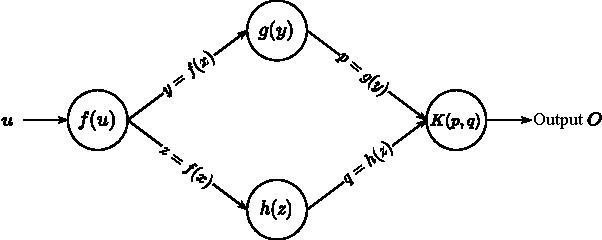
\includegraphics[width=0.7\textwidth]{thesis/figures/artificial-neural-network-backprop-example_cropped.pdf}
    \caption{A neural network with one input node, one hidden layer with two nodes and one output layer.}
    \label{fig:neural-network-example-backprop}
\end{figure}

In \cref{fig:neural-network-example-backprop}, we have a network with one input node (neuron), a hidden layer with two nodes and a single output layer with one node. We denote the input to the network as $u$, which is the product of the input data and the weights in the input layer. For the activation functions of the network, we denote them as $f$, $g$ and $h$. Moreover, we denote the results of the activation functions as $y$, $z$, $p$, $q$, and the function $K$ combines the result of $p$ and $q$ resulting in the output value $O$. We assume that we apply the weights of the hidden layer to the previous layer's output values during $g$ and $h$ and that we apply the weights of the output layer at $K$. The forward pass in this network is straightforward: We start the input node, pass the data on to $g$ and $h$ and combine the results in the output layer. Now, for the backwards pass, we first compute the loss at the output node using a loss function $L$. Furthermore, we compute the derivative of $L$ with respect to the input $u$. More formally, we compute
\begin{align}
    \parder{L}{u}
    &= \parder{L}{O} \cdot \parder{O}{u} \label{eqn:derivative-of-l-wrt-u} \\
    &= \parder{L}{O} \cdot \left[
    \parder{O}{p} \cdot \parder{p}{u} +
    \parder{O}{q} \cdot \parder{q}{u}
    \right] \text{(chain rule)} \notag \\
    &= \parder{L}{O} \cdot \left[
    \parder{O}{p} \cdot \parder{p}{y} \cdot \parder{y}{u} + 
    \parder{O}{q} \cdot \parder{q}{z} \cdot \parder{z}{u}
    \right] \text{(chain rule)} \notag \\
    &= \parder{L}{O} \cdot \left[
    \undertext{\parder{K(p, q)}{p} \cdot g'(y) \cdot f'(u)}{Path on top} + 
    \undertext{\parder{K(p, q)}{q} \cdot h'(z) \cdot f'(u)}{Path on bottom} \notag
    \right].
\end{align}
In \cref{eqn:derivative-of-l-wrt-u}, we see how to calculate the derivatives for a relatively small neural network. There exists, effective and more general frameworks to derive the derivative of the loss with respect to the input values, but we leave those details out and kindly refer the reader to \cite[Chapter 1.3]{Aggarwal18} for more details.

We have now gone over the forward and backward passes, which are the first two steps of the so-called \textit{backpropagation} algorithm. The remaining step of the algorithm is to use the computed derivatives to update the weights of the ANN. To do this, we use the \textit{gradient descent} (GD) algorithm. The main idea of gradient descent is to update the weights iteratively by moving them in the opposite direction of the gradient (i.e. the steepest descent) of the loss with respect to the weights. By doing so, it leads to better-fitting weights for the input-output data. In standard gradient descent, we perform its steps by
\begin{align}
    W \Leftarrow W - \alpha \cdot \parder{L}{W},
\end{align}
where $W = \left( w_1, w_2, \ldots, w_d \right)$ is the matrix consisting of the $d$ weights of an ANN. The learning rate $\alpha$ is a hyperparameter and determines how much learning we want to do in each step. The learning rate is usually set to a relatively low value, in the order of $10^{-2}$ to $10^{-5}$. We illustrate the effect of the gradient descent algorithm with a small example in \cref{fig:gradient-descent-example}, where we compute gradient descent for the paraboloid $f(x, y) = (x - 2)^2 + (y - 4)^2$. We set the starting point to be (-5, -10), the learning rate $\alpha$ to 0.05 and use 100 iterations. In \cref{fig:gradient-descent-example}, we see that the gradient descent algorithms finds the minimum of $f(x, y)$ relatively fast.
\begin{figure}[H]
    \centering
    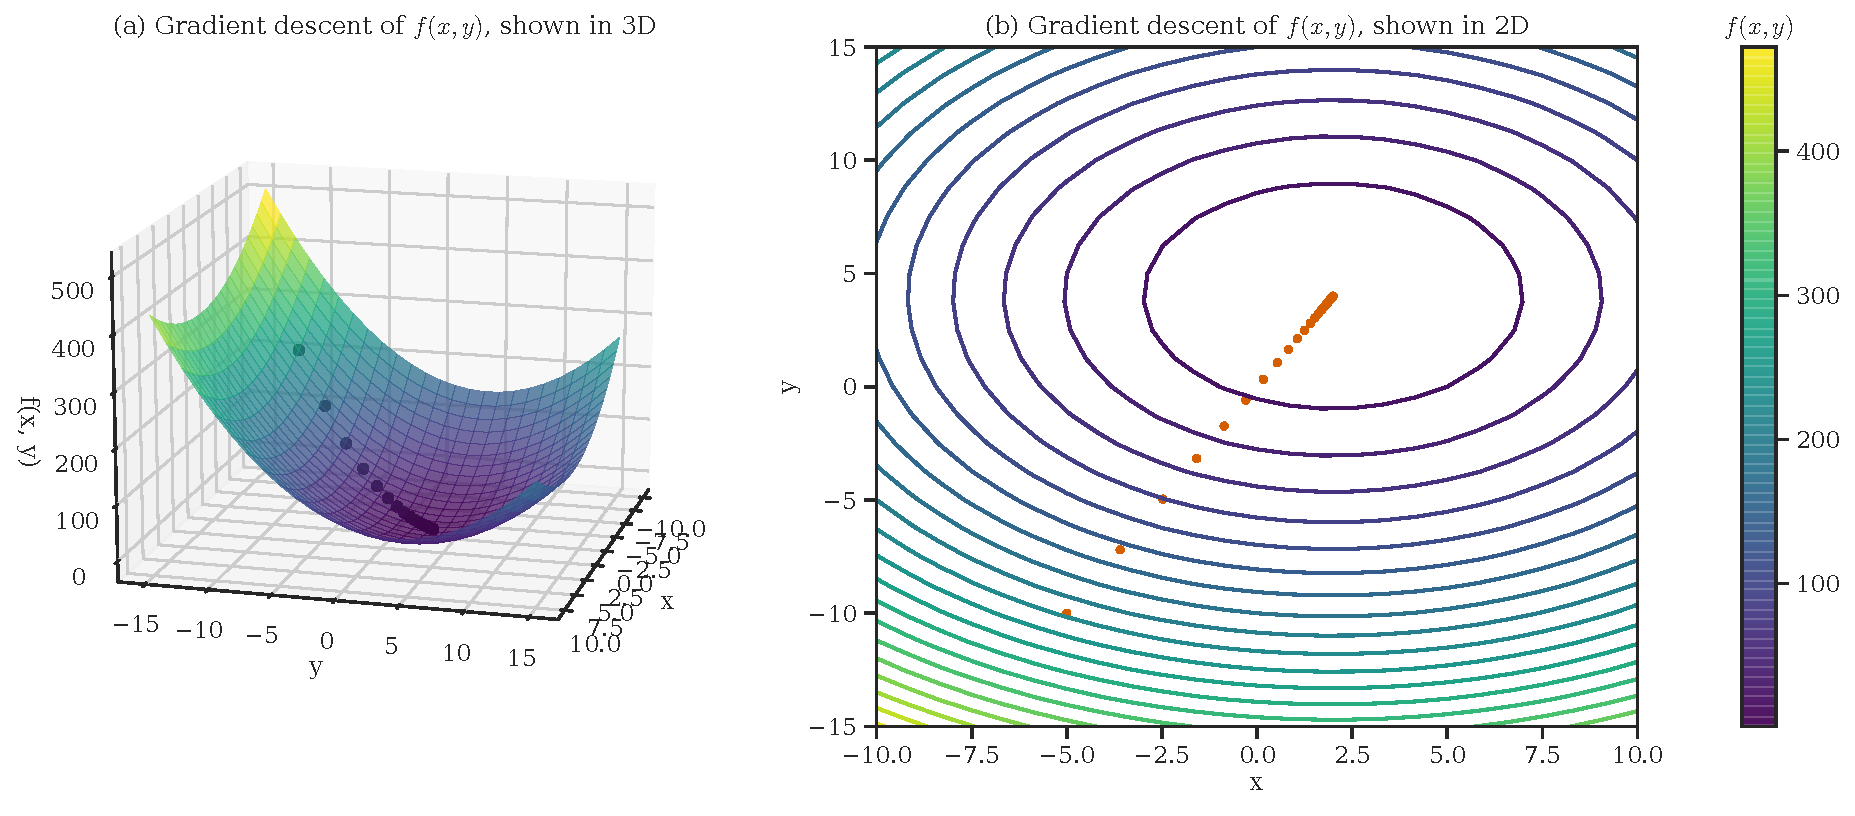
\includegraphics[width=\textwidth]{gradient-descent-example}
    \caption{Gradient descent of the function $f(x, y) = (x - 2)^2 + (y - 4)^2$. We start at point (-5, -10), use a learning rate $\alpha$ of 0.05 and compute for 100 iterations.}
    \label{fig:gradient-descent-example}
\end{figure}

Even though gradient descent works great for small applications, once we scale the number of parameters (weights) in the ANN to the more extremes (e.g. in the order of millions), it becomes impractical to compute for the entire training data at once. Furthermore, we observe that a loss function $L$ usually can be written as a sum of the loss of the individual training data points, where $L_i$ is the loss for training data point $i$. Thus, we define the individual loss $L_i$ as
\begin{align}
    \label{eqn:loss-function-sum-individual}
    L = \sumlim{i=1}{n} L_i.
\end{align}
Using the observation that we are able to write the loss function as the sum in \cref{eqn:loss-function-sum-individual}, we introduce the \textit{stochastic gradient descent} (SGD) method. Instead of performing gradient descent on the whole input data, SGD performs gradient descent for each input data separately. More formally, SGD performs its steps by
\begin{align}
    \label{eqn:sgd}
    W \Leftarrow W - \alpha \cdot \parder{L_i}{W},
\end{align}
where $n$ is the number of input data points and $L_i$ represents the loss of the $i$th input. We call SGD stochastic because a random sample of the training data is chosen for each iteration. An advantage that SGD has over GD, is that it runs a lot faster, at the expense of greater loss. Thankfully, there exists a variant of SGD which seeks to find a balance between speed and loss, namely the \textit{mini-batch stochastic gradient descent} (mini-batch SGD) method. In mini-batch SGD, we use a batch $B=\enclc{j_1, \ldots, j_m}$ of input training data indices when computing the weight updating. In other words, mini-batch SGD performs its steps by
\begin{align}
    \label{eqn:mbsgd}
    W \Leftarrow W - \alpha \cdot \sumlim{j \in B}{} \parder{L_j}{W}.
\end{align}
Mini-batch SGD often finds the best trade-off between stability, speed and memory requirements. However, we note that the memory requirement increases with the use of mini-batches. This is because we have to store bigger matrices in memory during training. We typically choose batch sizes that are a power of 2 (e.g. 32, 64, 128 or 256), as most modern hardware architectures optimize for such values.

In addition to the different variants of gradient descent, there exist a bunch of other variants which can solve issues such as getting stuck in local minima or speeding up the training process. We leave out the technical details of all these strategies here, but kindly refer the reader to \cite[Chapter 3.5]{Aggarwal18} for more details.

\subsection{Intrinsic dimension estimation}
\label{sec:intrinsic-dimension-estimation}
In machine learning, the \textit{manifold hypothesis} states that, in general, real-life high-dimensional data tends to live on a low-dimensional submanifold embedded within the high-dimensional space \cite[p. 16]{bengio2014representation}. To understand more about the underlying structure of the data we are working with, we can estimate the dimension of the low-dimensional submanifold. We call the process of estimating the dimension of the low-dimensional submanifold \textit{intrinsic dimension (ID) estimation}. More generally, a $D$-dimensional data set $X \in \R^D$ is said to have an ID equal to $d$ if $X$ lies entirely within a $d$-dimensional subspace of $\R^D$ \cite{lee2015intrinsic}. We separate between \textit{global} and \textit{local} ID estimation methods, where global methods estimate the ID for the entire data set, and local methods estimate ID for each data point in the data set. We note, however, that it is fully possible and common in the literature to approximate local ID estimates by computing global ID estimates of a $k$-nearest neighbourhood around each data point $x \in X$. In the following sub-subsections, we introduce five methods for estimating the ID. We leave out the technical details of the ID estimation methods, as they are not the focus of this thesis. Instead, we give an overall explanation for each of the methods, and kindly refer the reader to the source of each method for more details. For each of the methods we describe below, we assume that we have some data set $X \in \R^{N \times D}$ consisting of $N$ samples, where each sample is a $D$-dimensional vector. We base this subsection on \cite{lee2015intrinsic} if we do not state otherwise. Following, our interest is mainly in local ID estimation methods for this thesis, as we will use them for the analysis of word embeddings (\cref{sec:word-embeddings}) in \cref{sec:analysis-of-embeddings-intrinsic-dimension-estimation} and for polysemous word prediction in \cref{sec:analysis-of-embeddings-supervised-polysemy-prediction}.

\subsubsection{LPCA}
\label{sec:id-estimation-lpca}
One of the first and most simple kinds of ID estimation algorithm bases itself on the PCA algorithm (see \cref{sec:pca}). In particular, the ID estimation algorithm uses information from the eigenvalue decomposition of PCA to estimate the intrinsic dimension. We refer to this ID estimation algorithm as the \textit{local PCA} (LPCA) method, which was first introduced in \cite{Fukunaga1971}. We refer to \cite{Fukunaga1971} when explaining the LPCA method. The LPCA method works as follows. First, we reduce the dimensionality of the original data set $X$ from $D$ dimensions to $\hat{d}$ dimensions, by applying PCA and making sure that most of the variance in the $\hat{d}$ dimensions are kept. To select $\hat{d}$, LPCA counts the number of eigenvalues that are greater than a portion $\alpha$ of the largest eigenvalue, from PCAs eigenvalue decomposition. A typical value for $\alpha$ is 0.1, meaning that $\hat{d}$ is set to the number of eigenvalues that are greater than 90\% of the largest eigenvalue. The value $\hat{d}$ is then the estimated ID. The LPCA algorithm for estimating ID is a local estimator, meaning that estimates the ID for every data point $x \in X$. We typically implement LPCA using $k$-nearest neighbour, meaning that for every data point $x \in X$, we compute PCA of the $k$-nearest neighbourhood around $x$ to estimate its ID.

\subsubsection{KNN}
\label{sec:id-estimation-knn}
A popular approach to estimate the ID is to use $k$-nearest neighbour ($k$-NN) graphs. In this sub-subsection, we explain the \textit{$k$-NN algorithm} for ID estimation, as explained by \cite[p. 651]{Carter2010}. The $k$-NN algorithm uses the notion of the total edge length of the $k$-NN graph built on the data $X$, to estimate the ID $\hat{d}$. Let $D(x_i, x_j)$ denote the distance between two data points $x_i, x_j \in X$, and let $\mathcal{N}_{k, i}$ denote the set of the $k$-nearest neighbours of data point $x_i$. Then, we define the total edge length of the $k$-NN graph as
\begin{align}
    L_{\gamma, k}(X) = \sumlim{i=1}{n} \sumlim{y \in \mathcal{N}_{k, i}}{} D(x_i, x_j)^\gamma,
    \label{eqn:k-nn-id-estimation-l}
\end{align}
where $\gamma>0$ is a constant, weighting the distances between the data points in the $k$-NN graph. If we let $\gamma>1$, then we emphasize big distances between data points. The authors of \cite[p. 651]{Carter2010} then argue that, assuming the manifold hypothesis holds for the data $X$ (i.e. that the data $X$ can be fully described using a submanifold $X' \in \R^{N \times d}$), it is possible to estimate $\hat{d}$ by applying non-linear least squares to an approximation of the total edge length. The $k$-NN algorithm for estimating ID is a global estimator, meaning that estimates the ID of the whole data $X$. It is possible to make it local by applying the procedure we explained in the introduction to ID estimation in \cref{sec:intrinsic-dimension-estimation}.

\subsubsection{TWO-NN}
\label{sec:id-estimation-twonn}
Estimating the ID can be a hard task, especially if the underlying manifold of the data is twisted and curved. It is for this reason, the authors of \cite{Facco2017twonn} propose a two nearest neighbours estimator for ID estimation, which we refer to as the \textit{TWO-NN} method. TWO-NN uses the first and the second nearest neighbour of each data point in $X$ to estimate the ID. The authors of \cite{Facco2017twonn} show that by using the ratio of the distance to the second nearest neighbour to the first one to create a linear regression model which estimates the ID $\hat{d}$. Following, the authors claim that this minimality reduces the effect of complex manifolds, varying density and reduces the computational cost. The TWO-NN algorithm for estimating ID is a global estimator, meaning that estimates the ID of the whole data $X$. It is possible to make it local by applying the procedure we explained in the introduction to ID estimation in \cref{sec:intrinsic-dimension-estimation}.

\subsubsection{MLE}
\label{sec:id-estimation-mle}
Maximum likelihood estimation (MLE) is a method for estimating the parameters of a probability distribution, by either maximizing a likelihood function. \cite{Levina2004} propose a method that uses MLE to estimate the ID of data points $x \in X$. The idea is to estimate the ID locally, by assuming that the density $f(x)$ is constant for a small sphere $S_x(R)$ of radius $R$ around $x$. Then, they use a Poisson process to measure the rate of the counting process $N(t, x)$ which measures the number of points falling onto the sphere $S_x(R)$ at time $t$. Furthermore, they use MLE on the Poisson process to estimate the local ID $\hat{d}$ for point $x$. Note that in practice, it is common to use $k$-nearest neighbours instead of radius $R$ to find neighbours of $x$. An extension of the MLE method for estimating local ID was proposed by \cite{Haro2008}, which makes the ID estimator more robust to noise.

\subsubsection{TLE}
\label{sec:id-estimation-tle}
\textit{Tight Local Intrinsic Dimensionality Estimator} (TLE) \cite{Amsaleg2019} is a method for estimating the local ID of data points $x \in X$. The authors of TLE claim that the method works well in tight localities, i.e. within neighbourhoods of small size (e.g. using $k$-nearest neighbour). By using distances from $x$ to its $k$-nearest neighbours, TLE estimates the local ID $\hat{d}$. The authors of \cite{Amsaleg2019} claim that TLE can achieve more accurate ID estimates within small neighbourhoods around $x$ (i.e. for small values of $k$), which again can improve the quality of algorithms that depend on local ID estimates.

\subsection{Regression analysis}
\label{sec:regression-analysis}
\textit{Regression analysis} is a set of methods from statistics that estimate relationships between a \textit{dependent variable} and one or more \textit{independent variables}. To give an example, a dependent variable could be "income" and independent variables could be "education" and "experience". Regression analysis could help us to understand how income is affected by education, for instance. In this subsection, we look at three regression methods in particular: linear regression, lasso regression and logistic regression. We refer to \cite{James2013,fox2015applied} when describing concepts from regression analysis. Furthermore, we will use the lasso and logistic regression methods for the prediction of polysemous words in \cref{sec:analysis-of-embeddings-supervised-polysemy-prediction}.

\subsubsection{Linear regression}
\label{sec:linear-regression}
\textit{Linear regression}, as the name suggests, attempts to find linear relationships between variables. The simplest form of linear regression is between a dependent variable $X$ and a single independent variable $Y$. First, we assume that there is an approximately linear relationship between $X$ and $Y$. Then, we model the linear relationship as
\begin{align}
    Y \approx \beta_0 + \beta_1 X,
\end{align}
where the approximate equals sign "$\approx$" means that we are \textit{regressing} $Y$ onto $X$. The two constants $\beta_0$ and $\beta_1$ are unknown and represents the \textit{intercept} and \textit{slope} in terms of the linear model. We refer these two constants as the \textit{model parameters}. Following, we use some training to compute estimates of the models parameters, $\hat{\beta_0}$ and $\hat{\beta_1}$. We use the \textit{hat} symbol, $\string^$\,, to denote some estimated or predicted value. To predict future values for $Y$, we use the estimated parameters $\hat{\beta_0}$ and $\hat{\beta_1}$ by computing
\begin{align}
    \hat{Y} = \hat{\beta_0} + \hat{\beta_1}X,
    \label{eqn:y-hat-simple}
\end{align}
where $\hat{Y}$ is the predicted value of $Y$. To estimate the model parameters $\hat{\beta_0}$ and $\hat{\beta_1}$, we must use some training data. Now, we let $X = (x_1, x_2, \ldots, x_n) \in \R^n$ and $Y = (y_1, y_2, \ldots, y_n) \in \R^n$ represent our data as two $n$-dimensional vectors. In machine learning terms, we are in a supervised setting, since we know the true labels $y$ before trying to predict them. After applying some linear algebra, we rewrite $\cref{eqn:y-hat-simple}$ for a single data point $i$ as
\begin{align}
    \hat{y_i} =
        \begin{bmatrix}
            1 & x_i
        \end{bmatrix}
        \begin{bmatrix}
            \hat{\beta}_0 \\
            \hat{\beta}_1 \\
        \end{bmatrix},
    \label{eqn:y-hat-two-matrix-form-single-point}
\end{align}
where $\hat{y_i}$ is the predicted value for $x_i$. Since we have $n$ values for $X$ and $Y$, we need $n$ equations similar to \cref{eqn:y-hat-two-matrix-form-single-point}, which we combine into a single matrix equation as
\begin{align}
    \hat{Y} =
        \undertext{
        \begin{bmatrix}
            1 & x_1 \\
            1 & x_2 \\
            \vdots & \vdots \\
            1 & x_n \\
        \end{bmatrix}
        }{$X'$}
        \undertext{
        \begin{bmatrix}
            \hat{\beta}_0 \\
            \hat{\beta}_1 \\
        \end{bmatrix}
        }{$\hat{\beta}$},
    \label{eqn:y-hat-two-matrix-form}
\end{align}
where $X'$ is the \textit{model matrix}, consisting of ones in the first column and $X$ in the second column, and $\hat{\beta} = \enclp{\hat{\beta_0}, \hat{\beta_1}}$ is a vector consisting of the models parameters. Using the \textit{ordinary least squares} (OLS) method \cite[p. 208]{fox2015applied}, we get a closed-form expression for estimating the parameters $\hat{\beta}$, by computing
\begin{align}
    \hat{\beta} = \enclp{\trans{X'} X'}^{-1} \trans{X'}Y.
    \label{eqn:ordinary-least-squares}
\end{align}
The OLS method minimizes the \textit{residual sum of squares} (RSS), i.e. the sum of the squared differences between the true value $y$ and predicted value $\hat{y}$. More formally, we define the objective of OLS as
\begin{align}
    \text{RSS} = \sumlim{i=1}{n}{\enclp{y_i - (\hat{\beta_0} + \hat{\beta_1}x_i)}^2}.
    \label{eqn:RSS-ols-two-variables}
\end{align}
We illustrate the use of OLS in \cref{fig:linear-regression-ols}, where see a clear relationship between the variables $X$ and $Y$.
\begin{figure}[H]
    \centering
    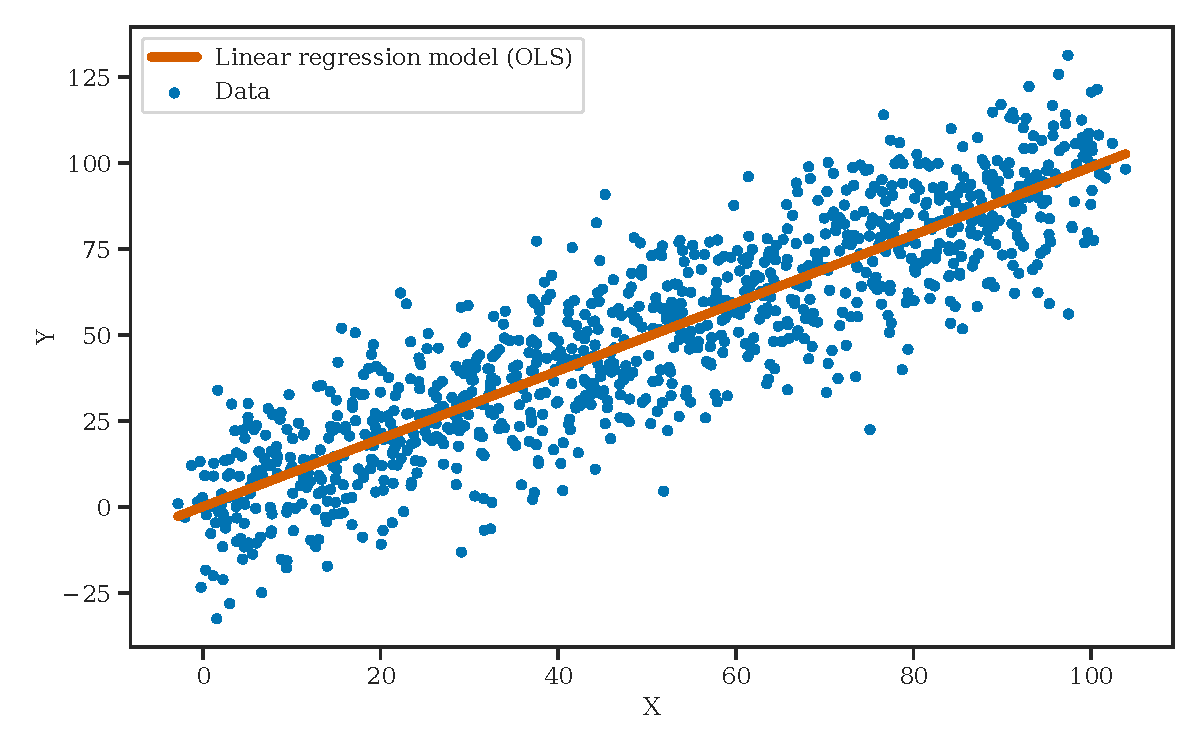
\includegraphics[width=0.7\textwidth]{thesis/figures/linear-regression-example.pdf}
    \caption{A linear regression model using OLS, with one dependent variable Y and one independent variable $X$. The red line shows the OLS model.}
    \label{fig:linear-regression-ols}
\end{figure}

So far, we have only looked at the simplest form of linear regression, namely only using a single independent variable $X$ to predict a value for $Y$. To generalize the linear regression to $k$ independent variables, we now assume that our training data has $k$ variables (which we also refer to as \textit{features} or \textit{columns}), i.e. $X \in R^{n \times d}$. Finally, we add the new columns from $X$ to the model matrix $X'$, by extending \cref{eqn:y-hat-two-matrix-form} as
\begin{align}
    \hat{Y} =
        \undertext{
        \begin{bmatrix}
            1 & x_{11} & \ldots & x_{1k} \\
            1 & x_{21} & \ldots & x_{2k} \\
            \vdots & \vdots & & \vdots \\
            1 & x_{n1} & \ldots & x_{nk} \\
        \end{bmatrix}
        }{$X'$}
        \undertext{
        \begin{bmatrix}
            \hat{\beta}_0 \\
            \hat{\beta}_1 \\
            \vdots \\
            \hat{\beta}_k \\
        \end{bmatrix}
        }{$\hat{\beta}$}.
    \label{eqn:y-hat-matrix-form-general}
\end{align}
To estimate the model parameters $\hat{\beta}$, we compute them using \cref{eqn:ordinary-least-squares}. Furthermore, we generalize the minimization objective of OLS in \cref{eqn:RSS-ols-two-variables} to use $k$ independent variables as well, by computing
\begin{align}
    \text{RSS} = \sumlim{i=1}{n}{\enclb{y_i - \enclp{\hat{\beta_0} +  \sumlim{j=1}{k}{\hat{\beta_j}x_{ij}}}}^2}.
    \label{eqn:RSS-ols-k-variables}
\end{align}

\subsubsection{Lasso regression}
\label{sec:lasso-regression}
Linear regression suffers from the fact that it has to use all independent variables to predict a value for the dependent variable. Imagine that we gather some $5$-dimensional data $X$, and want to predict some quantity $y$ using $X$. We perform some analysis on the data and notice that two of the features of the data are plain noise and most likely does not help to predict $y$. \textit{Lasso regression} is a slight modification of linear regression that helps us with this problem. By adding a \textit{penalty term} on the model parameters in the objective of the linear regression, lasso regression can push certain features to 0, essentially "removing" them from the model. If we have two similar features, the lasso is also able to "nullify" one of them, since the first one "explains" the second one. As a result, the models we get from lasso regression are generally much easier to interpret. What we have described here is also referred to as \textit{feature selection}, where the model automatically selects which variables are useful for prediction.

Lasso regression minimizes the residual sum of squares (RSS) plus some constant $\lambda$ times the \textit{$\ell_1$-norm} of the model parameters $\beta$. We define the minimization objective as
\begin{align}
    \sumlim{i=1}{n}{\enclb{y_i - \enclp{\hat{\beta_0} +  \sumlim{j=1}{k}{\hat{\beta_j}x_{ij}}}}^2} + \lambda ||\beta||_1 = \text{RSS} + \lambda ||\hat{\beta}||_1,
    \label{eqn:lasso-regression-objective}
\end{align}
where $\lambda \geq 0$ is a \textit{regularization} parameter. We denote the second term of \cref{eqn:lasso-regression-objective}, $\lambda ||\hat{\beta}||_1$, as the $\ell_1$-penalty, which is small when $\hat{\beta}_0$, $\hat{\beta}_1$, \ldots, $\hat{\beta}_k$ are small. When $\lambda = 0$, the penalty term has no effect and lasso regression produces the same result as standard linear regression. As $\lambda \rightarrow \infty$, the effect of the $\ell_1$-penalty grows and the model parameters $\hat{\beta}$ approaches zero, and in some cases, some of the model parameters are be exactly zero. We define the $\ell_1$-norm as $||\hat{\beta}||_1 = \sum |\hat{\beta}_j|$, where $|\cdot|$ is the absolute value.

\subsubsection{Logistic regression}
\label{sec:logistic-regression}
When describing linear regression models in \cref{sec:linear-regression}, we assume that the response variable $Y$ is \textit{quantitative}. When working with \textit{qualitative} data, on the other hand, linear regression fails to work. For example, colours are qualitative, taking on values such as blue, red, green or brown; we can not claim that red is greater than blue or brown is less than green (discarding RGB colour information). When we predict a qualitative response variable $Y$ using some data $X$, we perform what we call a \textit{classification} task. \textit{Logistic regression} is a method that can predict the response variable $Y$ when it falls into one of two categories (i.e. binary response). Examples of a binary response variable are "Yes"/"No", "Is a dog"/"Is not a dog" and the typical 0/1, which we commonly use in machine learning. Logistic regression creates a model that models the probability that $Y$ falls belong to a particular category. In \cref{fig:logistic-regression-example}, we further motivate the use of logistic regression for binary-response tasks and we see that linear regression is not well-suited for predicting values between 0 and 1.
\begin{figure}[H]
    \centering
    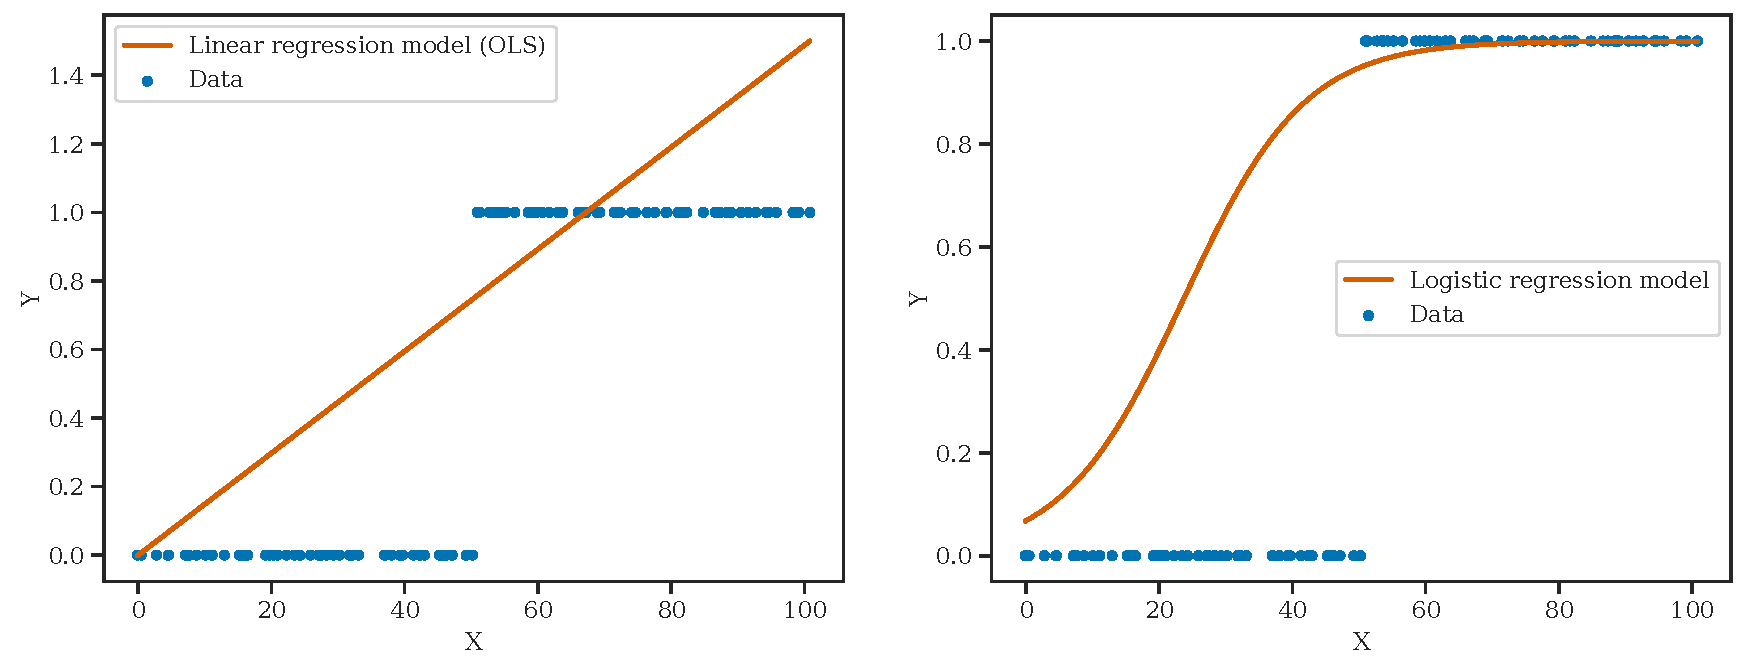
\includegraphics[width=\textwidth]{thesis/figures/logistic-regression-example.pdf}
    \caption{Illustration of linear and logistic regression models predicting some binary response variable $Y$ on data $X$. We see that logistic regression is particularly well-suited for predicting values for $Y$ between 0 and 1. Linear regression fails to model this relationship and even goes out of bounds for $X > 70$.}
    \label{fig:logistic-regression-example}
\end{figure}

Let $p(X) = Pr(Y = 1|X)$ denote the probability of $Y$ being 1 when we have the data $X$. If we want to model this relationship, we could use linear regression by
\begin{align}
    p(X) = \beta_0 + \beta_1 X.
\end{align}
Unfortunately, as mentioned earlier, linear regression is not a good fit for such problems and we would have the situation on the left of \cref{fig:logistic-regression-example}. In logistic regression, the \textit{logistic function} is used to ensure that the output value falls between 0 and 1, and we define it as
\begin{align}
    p(X) = \frac{\exp{\enclp{\beta_0 + \beta_1 X}}}{1 + \exp{\enclp{\beta_0 + \beta_1 X}}}.
    \label{eqn:logistic-function-p-x}
\end{align}
The plot to the right of \cref{fig:logistic-regression-example} shows the effect of the logistic function, creating an S-shaped like curve that, for high values of $X$, creates values close to, but never greater than 1. On the other hand, the logistic function creates values close to, but lever less than 0 for low values of $X$. Manipulating \cref{eqn:logistic-function-p-x} a bit, we get that
\begin{align}
    \frac{p(X)}{1 - p(X)} = \exp{\enclp{\beta_0 + \beta_1 X}},
    \label{eqn:logistic-function-odds}
\end{align}
where we refer the left-hand-side of \cref{eqn:logistic-function-odds}, i.e. $p(X)/\enclb{1 - p(X)}$, as the \textit{odds}. As $p(X)$ increases, the odds increases exponentially towards $\infty$. Taking the logarithm of both sides of \cref{eqn:logistic-function-odds}, we finally arrive at
\begin{align}
    \log \enclp{\frac{p(X)}{1 - p(X)}} = \beta_0 + \beta_1 X,
    \label{eqn:logistic-function-logit}
\end{align}
where we refer the left-hand-side of \cref{eqn:logistic-function-logit} as the \textit{logit}. Thus, we see that the logistic regression model has a logit that is linear in $X$. If we increase $X$ by one unit, then the log odds increase by $\beta_1$. However, note that the relationship between $p(X)$ and $X$ in \cref{eqn:logistic-function-p-x} is not a straight line. For this reason, the amount of $p(X)$ changes due to a single unit change in $X$ depends on the current value of $X$. In \cref{fig:logistic-regression-example}, we see that once $X$ reaches a certain threshold (e.g. $X=30$), the rate at which $Y$ changes decreases towards zero.

If we would like to model logistic regression using multiple predictors, we only have to perform a simple extension from simple to multiple linear regression. We generalize \cref{eqn:logistic-function-logit} as
\begin{align}
    \log \enclp{\frac{p(X)}{1 - p(X)}}
    &= \beta_0 + \beta_1 X_1 + \beta_2 X_2 + \ldots + \beta_k X_k \label{eqn:logistic-function-logit-multiple} \\
    &= \beta_0 + \sumlim{i=1}{k}{\beta_i X_i}, \notag
\end{align}
where $X = \enclp{X_1, X_2, \ldots, X_k}$ are $k$ predictors.

To estimate the parameters $\beta_0, \beta_1, \ldots, \beta_k$ for $k$ predictors, it is common to use the \textit{maximum likelihood} method. We do not go into detail about the maximum likelihood method here, but kindly refer the reader to \cite[p. 214]{fox2015applied} for more details.

\subsection{Model selection}
\label{sec:model-selection}
\textit{Model selection} is an important aspect of modern machine learning. When working with machine learning, we would like to understand which model solves the problem the best, and model selection helps us with this. Model selection is the task of selecting a model for a particular problem using the data at hand. We look at a couple of methods for performing model selection, namely using train/validation/test splits and $K$-fold cross-validation. We refer to \cite{James2013} when describing model selection methods. Furthermore, we will use model selection when training lasso and logistic regression model for supervised word polysemy prediction in \cref{sec:analysis-of-embeddings-supervised-polysemy-prediction}.

\subsubsection{Train, validation and test splits}
\label{sec:train-val-test-splits}
When training a supervised machine learning model, we typically have some data $X$ and corresponding labels $y$. The task is to predict the labels $y$ using the data $X$. Since we do not know apriori which model or model parameters to use, the most common way to figure this out is by performing model selection. The simplest kind of model selection for machine learning models is to split the data $X$ and labels $y$ into three data sets, namely the \textit{train-}, \textit{validation-}, and \textit{test data sets}. The new data sets are chosen at random and do not overlap. An example of a train/validation/test split ratio could be 80/10/10, where we use 80\% of the data in the training data set, 10\% of the data in the validation data set and 10\% of the data in the test data set. Exactly how we split the data sets into the smaller train/validation/test data sets depends on the application and how much data we are working with. In more modern machine learning models, e.g. using artificial neural networks, it is common to use up to 99\% of the data for training, as long as we have a big enough data set (e.g. $>1$ million data points).

We use the train data set to learn the models' parameters from the data, e.g. a linear regression models $\beta$ parameter. The train data set is usually much larger than the validation or test data sets. To evaluate the parameters of the model, we use the \textit{validation data set}. When we evaluate a trained model using a validation data set, we perform what we call the \textit{validation set approach}. The validation data set provides an unbiased estimate of a models' fit on the training data set while tuning some \textit{hyperparameter}. A hyperparameter is a parameter that we choose for the model beforehand, in contrast to a model parameter, which the model learns internally. Tuning hyperparameters can be a difficult task, especially if we have a lot of hyperparameters with various values. A typical way of performing hyperparameter optimization is by using \textit{grid search}, which tries out all combinations of all hyperparameter values. Grid search can be computationally expensive, especially if we would like to try out many choices of hyperparameters. For this reason, we typically use grid searches to find potential ranges where the optimal hyperparameters live and then narrow down the search for smaller ranges of hyperparameters to find more optimal ones.

After selecting a model or a set of model parameters using the validation data set, we use the test data set to give an unbiased estimate of how the model performs on unseen data. Additionally, we refer to the test data set as the \textit{hold-out data set}, because its only use is at the end of model selection. Note that we do not necessarily require to have a test data set available to perform model selection, as it only evaluates the performance of the final model. A common approach is also to exclude the test data set and instead split the original data $X$ into training and validation only. By doing so, we are unable to get an unbiased estimate of the models' performance on unseen data. We illustrate the process of splitting data into train/validation/test splits in \cref{fig:train-val-test-splits}.
\begin{figure}[H]
    \centering
    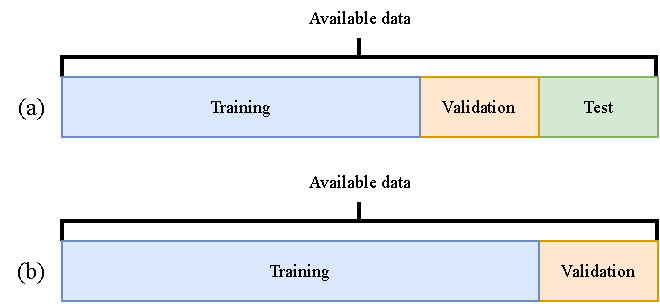
\includegraphics[width=0.9\textwidth]{thesis/figures/train-val-test-splits_cropped.pdf}
    \caption{Example of ways to partition a data set for model selection. The partition on the top (a) splits the data into training, validation and test, while the partition on the bottom (b) splits the data into training and validation only.}
    \label{fig:train-val-test-splits}
\end{figure}

The validation set approach is simple and works fine in practice. There are, however, a couple of drawbacks when using this method. Depending on which observations we include in the training and validation data sets, the validation estimate of the error can vary a lot. In addition to this, since the validation set approach only uses a subset of the observations to train the model, and the fact that statistical models perform worse when we train them on less data, the validation error rate tends to overestimate the test error rate of a model trained on the entire data set. In the next sub-subsection, we introduce $k$-fold cross-validation, an improvement over the validation set approach that addresses these two drawbacks.

\subsubsection{k-fold cross-validation}
\label{sec:cross-validation}
An alternative to the validation set approach is the \textit{$k$-fold cross validation} (CV) method. The $k$-fold CV method randomly divides the training data $X$ into $k$ groups, or \textit{folds}, of approximately equal size. We treat the first fold as the validation data set and train the model on the remaining $(k - 1)$ folds. We compute the validation error $\text{Err}_1$ on the first validation data set. Following, this procedure is repeated $k$ times, and for each time, we use a different group of data points from the original training data $X$ as the validation data. This results in $k$ estimates of the test error, i.e. $\text{Err}_1$, $\text{Err}_2$, \ldots, $\text{Err}_k$. We compute the total $k$-fold CV error estimate by taking the mean of these values, as
\begin{align}
    \text{CV}_k = \frac{1}{k} \sumlim{i=1}{k} \text{Err}_i.
\end{align}
Choosing a value for $k$ is a hard problem. The most common choice is to set $k=5$ or $k=10$, depending on the problem. We kindly refer the reader to \cite[Section 5.1.4]{James2013} for more details on choosing a value for $k$.

We show an illustrative example of $k$-fold CV in \cref{fig:k-fold-cv}, where we see a typical set-up when using a $k$-fold CV, namely to split all available data into training and test data sets. During the training process, the training data set is furthermore split into training and validation data sets for that particular $k$.
\begin{figure}[H]
    \centering
    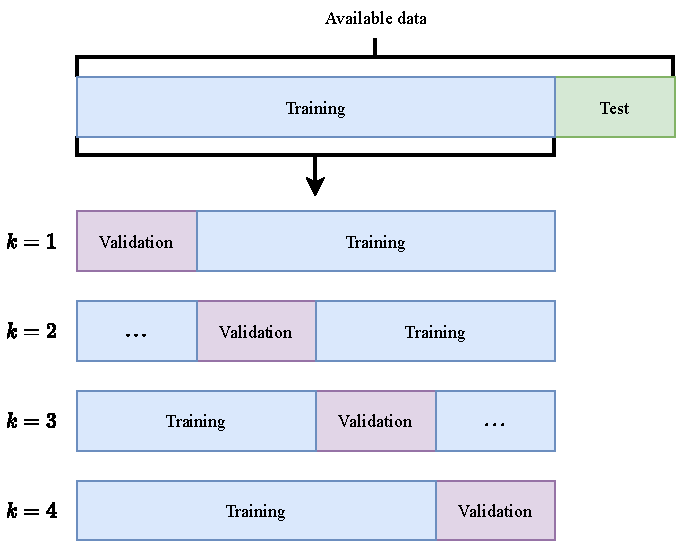
\includegraphics[width=0.9\textwidth]{thesis/figures/k-fold-cv_cropped.pdf}
    \caption{Data split into training and test data sets. To perform model selection, we use $k$-fold cross-validation. In this example, we have a $4$-fold cross-validation setting. As the $k$ increases, we have different data sets for both training and validation.}
    \label{fig:k-fold-cv}
\end{figure}

The benefit of using $k$-fold CV is that, by both training on different subsets of the training data and evaluating the model on different validation data sets, the estimated test error becomes more accurate and we get less varying results, as long as we select a good value for $k$.

\subsection{Performance metrics}
\label{sec:performance-metrics}
In this subsection, we introduce some common choices of performance metrics for regression and classification problems. We use performance metrics to evaluate machine learning models on data sets. In the following sub-subsections, we look at classification accuracy, the confusion matrix and sensitivity. Furthermore, we will use the performance metrics below to evaluate the word2vec model in \cref{sec:word2vec-model-evaluation} and for evaluating results from prediction of polysemous words in \cref{sec:analysis-of-embeddings-supervised-polysemy-prediction}.

\subsubsection{Classification accuracy}
\label{sec:classification-accuracy}
\textit{Classification accuracy} (which we also refer to as \textit{accuracy}) is the ratio between correct predictions to the total number of samples. We typically use classification accuracy in classification problems, as it is a simple and interpretable metric. Let $C_p$ be the number of correct predictions and let $N$ be the total number of samples. We compute classification accuracy as
\begin{align}
    \text{ACC}(C_p, N) = \frac{C_p}{N}.
    \label{eqn:classification-accuracy}
\end{align}
One pitfall of using classification accuracy is when we are dealing with classification problems with unbalanced data sets. Imagine that we want to compute the performance of a classification model for classifying whether or not a patient has a rare but fatal disease. If we use classification accuracy, it is not uncommon to see high accuracies (e.g. $99.9\%$), when in reality, the number of correct classifications for whether or not a patient has the disease is significantly lower. In other words, we get a false sense of the models' performance. To deal with such cases, it is more common to use metrics such as sensitivity (see \cref{sec:sensitivity}), which deals with class imbalance much better and is well-suited for specific tasks.

\subsubsection{Confusion matrix}
\label{sec:confusion-matrix}
\textit{Confusion matrices} explains the performance of classification models by creating a matrix of predicted values to true labels. We see such a confusion matrix in \cref{fig:confusion-matrix}, where we have a binary classification problem (two classes; 0 and 1). As we see in \cref{fig:confusion-matrix}, we have four terms which describe the performance of the model, namely the \textit{True Negative} ($TN$), \textit{False Negative} ($FN$), \textit{False Positive} ($FP$) and \textit{True Positive} ($TP$) terms. $TN$ is the number of predicted negative classes when the true classes were negative, while on the other hand, $TP$ is the number of predicted positive classes when the true classes were positive. Off the diagonals of \cref{fig:confusion-matrix}, we see FP, which is the number of predicted positive classes when the true classes were negative, and FN, which is the number of predicted negative classes when the true classes were positive. When computing accuracy we would like, ideally, the number of $TN$ and $TP$ samples to be as high as possible and the number of $FN$ and $FP$ samples to be as low as possible. In cases where we have a high class imbalance (e.g. from example in \cref{sec:classification-accuracy}), it is more common to optimize either $TN$ or $TP$ to be as high as possible, effectively minimizing either $FN$ or $FP$. We look at one such metric, namely sensitivity in \cref{sec:sensitivity}.
\begin{figure}
    \centering
    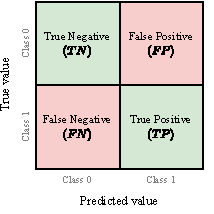
\includegraphics[width=0.5\textwidth]{thesis/figures/confusion-matrix_cropped.pdf}
    \caption{A typical example of a confusion matrix of a binary classification problem, with classes 0 and 1.}
    \label{fig:confusion-matrix}
\end{figure}

\subsubsection{Sensitivity}
\label{sec:sensitivity}
\textit{Sensitivity} is a performance metric which measures the ability of a classification model to correctly classify a positive class (e.g Class 1 in \cref{fig:confusion-matrix}). The sensitivity only focuses on the values where the true class is positive, i.e $FN$ and $TP$ for a binary classification problem. More formally, we define sensitivity as the portion of correctly predicted positive classes to the number of samples with a positive class. We compute the sensitivity as
\begin{align}
    \text{SEN} = \frac{TP}{TP + FN}.
    \label{eqn:sensitivity}
\end{align}
If we, on the other hand, would like to look at the ability of a classification model to correctly classify a negative class (e.g. Class 0 in \cref{fig:confusion-matrix}), we can, with minor modification of \cref{eqn:sensitivity}, change to focus on the prediction of negative classes. This modification creates a measure commonly referred to as \textit{specificity}.